\documentclass[utf8]{frontiersSCNS}

\setcitestyle{square}
\usepackage{url,hyperref,lineno,microtype,subcaption}
\usepackage[onehalfspacing]{setspace}

\usepackage{bm}
\usepackage[ruled,vlined]{algorithm2e}
\usepackage{graphicx}
\usepackage{amsmath}
\usepackage{amssymb}
\usepackage{mathtools}
\usepackage{adjustbox}
\usepackage{array}
\usepackage{float}
\usepackage{appendix}

\newcommand{\mtx}[1]{\bm{#1}}
\DeclareMathOperator*{\minimize}{minimize}
\newcolumntype{L}{>{\centering\arraybackslash}m{.3\textwidth}}
\renewcommand{\arraystretch}{1.4}
\SetArgSty{textnormal}

\linenumbers

\def\keyFont{\fontsize{8}{11}\helveticabold }
\def\firstAuthorLast{Gammell {et~al.}}
\def\Authors{Jimmy Gammell\,$^{1,*}$, Sonia M. Buckley\,$^{1}$,Sae Woo Nam\,$^{1}$ and Adam N. McCaughan\,$^{1}$}
\def\Address{$^{1}$National Institute of Standards and Technology, Boulder, CO, United States}
\def\corrAuthor{Jimmy Gammell}
\def\corrEmail{jimmy.gammell@colorado.edu}

\begin{document}
\onecolumn
\firstpage{1}

\title[Skip connections for equilibrium propagation]{Layer-skipping connections improve the effectiveness of equilibrium propagation on layered networks} 

\author[\firstAuthorLast ]{\Authors}
\address{}
\correspondance{}

\extraAuth{}% If there are more than 1 corresponding author, comment this line and uncomment the next one.
%\extraAuth{corresponding Author2 \\ Laboratory X2, Institute X2, Department X2, Organization X2, Street X2, City X2 , State XX2 (only USA, Canada and Australia), Zip Code2, X2 Country X2, email2@uni2.edu}


\maketitle


\begin{abstract}
\section{}
Equilibrium propagation is a learning framework that marks a step forward in the search for a biologically-plausible implementation of deep learning, and could be implemented efficiently in neuromorphic hardware. Previous applications of this framework to layered networks encountered a vanishing gradient problem that has not yet been solved in a simple, biologically-plausible way. In this paper, we demonstrate that the vanishing gradient problem can be overcome by replacing some of a layered network's connections with random layer-skipping connections. We additionally compare the computational complexities of equilibrium propagation and backpropagation to show that it would be easier to implement the former in neuromorphic hardware.

\tiny
 \keyFont{ \section{Keywords:} equilibrium propagation, deep learning, small-world, layer-skipping connections, neuromorphic computing, biologically-motivated}
 
\noindent\textbf{Number of words:} 3152

\noindent\textbf{Number of figures:} 7

\noindent\textbf{Number of tables:} 1
\end{abstract}

\section{Introduction}

As research into neural networks grows, there has been increased interest in designing biologically-inspired training algorithms, as they may offer insight into biological learning processes and also offer clues towards developing energy-efficient neuromorphic systems \citep{wozniak2018, crafton2019, ernoult2020, bartunov2018, lillicrap2014, bengio2015}. The equilibrium propagation learning framework developed \cite{scellier17} is one such algorithm.  It is a method for training a class of energy-based networks, the prototype for which is the continuous Hopfield network \cite{hopfield1984}.  In particular, it addresses one of the major issues that prevent other training algorithms (such as backpropagation) from being biologically-plausible, which is the requirement for separate computation pathways for different phases of training. This also makes the algorithm appealing for practical implementation into neuromorphic hardware, because only a single computation circuit is required within each (non-output) neuron, rather than multiple distinct circuits. However, current implementations of the algorithm still have a defect that diminishes its biological plausibility: they require hand-tuned per-layer hyperparameters to account for a vanishing gradient through the network. In addition to not being biologically plausible, these multiplicative hyperparameters would be difficult to implement in a neuromorphic hardware system with limited bit depth. In this work, we demonstrate that the vanishing gradient problem can instead be addressed through topological means: by randomly replacing some of a layered network's connections with layer-skipping connections, we can generate a network that trains each layer more evenly and does not need per-layer hyperparameters. This solution is biologically-plausible and would be easier to implement in a neuromorphic system; additionally, it entails hand-tuning only two new hyperparameters (the number of layer-skipping connections and their initial weights), whereas the original solution adds a new hyperparameter for each pair of layers in a network.


Implementation of equilibrium propagation in \citep{scellier17} was hindered by a vanishing gradient problem whereby networks with as few as 3 hidden layers trained slowly on MNIST \citep{mnist1998} -- a serious issue given that network depth is critical to performance on difficult datasets \citep{simonyan2014, srivastava2015tvdn} and that convergence to a low error rate on MNIST is a low bar to meet. The problem was overcome in \citep{scellier17} by independently tuning a unique learning rate for each layer in the network.  These learning rates were multiplicative factors that proportionally scaled the signals communicated between layers.



In our work, we have modified the strictly-layered topology of the original implementation by adding and removing connections to create a small-world-like network\citep{watts98}. Through this modification we have eliminated the per-layer hyperparameters without degrading the algorithm's performance -- the modified network produces 0\% training error (out of 50,000 examples) and $\lesssim$2.5\% test error (out of 10,000 examples) on MNIST using a network with three hidden layers and no regularization term in its cost function. These error rates are comparable to those of other biologically-motivated networks \citep{bartunov2018} and are approximately the same as those of the layered network with unique, manually-tuned learning rates in \citep{scellier17}. Our method could be implemented with relative ease in any system with configurable connectivity, such as those already described in several neuromorphic hardware platforms \citep{davies2018, schemmel2010, shainline2019}. Layer-skipping connections have been observed in biological brains \citep{bullmore2009}, so the approach is biologically-plausible. Similar techniques have seen success in convolutional \citep{he2015, srivastava2015} and multilayer feedforward \citep{xiaohu2011, krishnan2019} networks. Our findings outlined in this paper suggest that layer-skipping connections are effective-enough to be appealing in contexts where simplicity and biological plausibility are important. While small-world networks are not a novel concept, to our knowledge our work is the first to train small-world-like networks using the Equilibrium Propagation learning framework.

\section{Background}

\subsection{Equilibrium propagation}
\label{sec:eqp_formulation}

Similarly to backpropagation, the equilibrium propagation algorithm \citep{scellier17} trains networks by approximating gradient descent on a cost function. Equilibrium propagation is applicable to any network with dynamics characterized by evolution to a fixed point of an associated energy function; our implementation is a recreation of that in \citep{scellier17}, which applies it to a continuous Hopfield network \citep{hopfield1984}. The mathematical formulation of the framework can be found in \citep{scellier17}. We discuss its appeal over backpropagation in section \ref{sec:comparison}.

\subsubsection{Implementation in a continuous Hopfield network}

Here we summarize the equations through which a continuous Hopfield network is trained using equilibrium propagation; this summary is based on the more-thorough and more-general treatment in \citep{scellier17}.

Consider a network with $n$ neurons organized into an input layer with $p$ neurons, hidden layers with $q$ neurons and an output layer with $r$ neurons. Let the activations of these neurons be denoted respectively by vectors $\mtx{x}\in\mathbb{R}^{p}$, $\mtx{h}\in\mathbb{R}^{q}$ and $\mtx{y}\in\mathbb{R}^{r}$, and let $\mtx{s}=(\mtx{h}^{T},\mtx{y}^{T})^{T}\in\mathbb{R}^{q+r}$ and $\mtx{u}=(\mtx{x}^{T}, \mtx{s}^{T})^{T}\in\mathbb{R}^{n}$ be vectors of, respectively, the activations of non-fixed (non-input) neurons and of all neurons in the network. Let $\mtx{W}\in\mathbb{R}^{n\times n}$ and $\mtx{b}\in\mathbb{R}^{n}$ denote the network's weights and biases where $w_{ij}$ is the connection weight between neurons $i$ and $j$ and $b_i$ is the bias for neuron $i$ ($\forall i \;w_{ii}=0$ to prevent self-connections), and let $\rho$ denote its activation function; here and in \citep{scellier17},
\begin{equation}
\rho(x)=\begin{cases}0&x<0\\x&0\leq x\leq 1\\1&x>1\end{cases} \label{eqn:hardened_sigmoid}
\end{equation}
 is a hard sigmoid function
where $\rho'(0)=\rho'(1)$ is defined to be 1 to avoid neuron saturation. Let $\mtx{\rho}((x_1,\hdots, x_n)^T)=(\rho(x_1),\hdots,\rho(x_n))^T$.

The behavior of the network is to perform gradient descent on a total energy function $F$ that is modified by a training example $(\mtx{x}_d,\mtx{y}_d)$. Consider energy function $E:\mathbb{R}^n\to\mathbb{R}$,
\begin{equation}
E(\mtx{u}; \mtx{W}, \mtx{b})=\frac{1}{2}\mtx{u}^T\mtx{u}-\frac{1}{2}\mtx{\rho}(\mtx{u})^T \mtx{W} \mtx{\rho}(\mtx{u})-\mtx{b}^T\mtx{u} \label{eqn:energy}
\end{equation}
and arbitrary cost function $C:\mathbb{R}^r\to\mathbb{R}_{+}$; here and in \citep{scellier17} it is a quadratic cost function given by
\begin{equation}
C(\mtx{y})=\frac{1}{2}||\mtx{y}-\mtx{y}_d||_2^2, \label{eqn:cost}
\end{equation}
though the framework still works for cost functions incorporating a regularization term dependent on $\mtx{W}$ and $\mtx{b}$. The total energy function $F:\mathbb{R}^n\to\mathbb{R}$ is given by
\begin{equation}
F(\mtx{u}; \beta, \mtx{W}, \mtx{b})=E(\mtx{u};\mtx{W}, \mtx{b})+\beta C(\mtx{y}) \label{eqn:total_energy}
\end{equation}
where the clamping factor $\beta$ is a small constant. $\mtx{s}$ evolves over time $t$ as
\begin{equation}
\frac{d\mtx{s}}{dt}\propto -\frac{\partial F}{\partial \mtx{s}}. \label{eqn:dynamics}
\end{equation}
Equilibrium has been reached when $\frac{\partial F}{\partial \mtx{s}} \approx 0$. This can be viewed as solving the optimization problem
\begin{equation}
\minimize_{\mtx{s}\in\mathbb{R}^{q+r}}F((\mtx{x}_d^T,\mtx{s}^T)^T; \beta, \mtx{W}, \mtx{b}) 
\end{equation}
by using gradient descent to find a local minimum of $F$.

The procedure for training on a single input-output pair $(\mtx{x}_d,\mtx{y}_d)$ is as follows:
\begin{enumerate}
\item Clamp $\mtx{x}$ to $\mtx{x}_d$ and perform the free-phase evolution: evolve to equilibrium on the energy function $F(\mtx{u}; 0, \mtx{W}, \mtx{b})$ in a manner dictated by equation \ref{eqn:dynamics}. Record the equilibrium state $\mtx{u}^0$.
\item Perform the weakly-clamped evolution: evolve to equilibrium on the energy function $F(\mtx{u}; \beta, \mtx{W}, \mtx{b})$ using $\mtx{u}^0$ as a starting point. Record the equilibrium state $\mtx{u}^{\beta}$.
\item Compute the correction to each weight in the network: 
\begin{equation}
\Delta W_{ij}=\frac{1}{\beta}(\rho(u_i^\beta)\rho(u_j^\beta)-\rho(u_i^0)\rho(u_j^0)). \label{eqn:weight_correction}
\end{equation}
Adjust the weights using $W_{ij}\leftarrow W_{ij}+\alpha\Delta W_{ij}$ where the learning rate $\alpha$ is a positive constant.
\item Compute the correction to each bias in the network:
\begin{equation}
\Delta b_i=\frac{1}{\beta}(\rho(u_i^{\beta})-\rho(u_i^0)) \label{eqn:bias_correction}
\end{equation}
and adjust the biases using $b_i\leftarrow b_i+\alpha\Delta b_i$.
\end{enumerate}
This can be repeated on as many training examples as desired. Training can be done on batches by computing $\Delta W_{ij}$ and $\Delta b_i$ for each input-output pair in the batch, and correcting using the averages of these values. Note that the correction to a weight is computed using only the activations of neurons it directly affects, and the correction to a bias is computed using only the activation of the neuron it directly affects. This contrasts with backpropagation, where to correct a weight or bias $l$ layers from the output it is necessary to know the activations, derivatives and weights of all neurons between $0$ and $l-1$ layers from the output.

\subsection{Vanishing gradient problem}
\label{sec:vangrad}

Vanishing gradients are problematic because they reduce a network's rate of training and could be difficult to represent in neuromorphic analog hardware due to limited bit depth. As a simple example, the multiplicative factor of 0.008 used in previous implementations would lead to significant precision errors in a system with signals represented by integers from 0-16 (bit depth of 4).

The vanishing gradient problem is familiar in the context of conventional feedforward networks, where techniques such as the weight initialization scheme in \citep{glorot2010}, the use of activation functions with derivatives that do not lead to output saturation \citep{schmidhuber2015}, and batch normalization \citep{ioffe2015} have been effective at overcoming it. However, in the context of the networks trained in \citep{scellier17}, the vanishing gradient problem persists even when the former two techniques are used. To our knowledge batch normalization has not been used in the context of equilibrium propagation; however, it seems unlikely to be biologically-plausible.

\subsection{Related work}

References \citep{lee2015, xie2003, pineda1987} describe other approaches to locally approximating the gradient of a cost function. References \citep{lillicrap2014, crafton2019} explore the use of a random feedback matrix for backwards connections that is more biologically-plausible than identical forwards and backwards connections. Reference \citep{bartunov2018} explores the present state of biologically-motivated deep learning, and \citep{bengio2015} discusses the criteria a biologically-plausible network would need to satisfy. References \citep{shainline2019, davies2018, nahmias2013} discuss analog hardware that could potentially implement equilibrium propagation. References \citep{he2015, srivastava2015, xiaohu2011, krishnan2019} use layer-skipping connections for other types of networks and learning frameworks. References \citep{ioffe2015, glorot2010} give approaches to solving vanishing gradient problems.

\section{Implementation}
\label{sec:implementation}

We implemented \footnote{\url{https://github.com/jgammell/Equilibrium_Propagation_mobile.git}} the Equilibrium Propagation framework described in \citep{scellier17} using Pytorch \citep{pytorch2019}. Like the networks in \citep{scellier17}, our networks are continuous Hopfield networks with a hard sigmoid activation function $$\sigma(x)=\text{Max}\{0, \text{Min}\{x, 1\}\}$$ and squared-error cost function with no regularization term $$C=||\mtx{y}-\mtx{y}_d||_2^2,$$ where $\mtx{y}$ is the network's output and $\mtx{y}_d$ is the target output.

We use two performance-enhancing techniques that were used in \citep{scellier17}: we randomize the sign of $\beta$ before training on each batch, which was found in the original paper to have a regularization effect, and we use persistent particles, where the state of the network after training on a given batch during epoch $n$ is used as the initial state for that batch during epoch $n+1$. Persistent particles reduce the computational resources needed to approximate the differential equation governing network evolution, and would be unnecessary in an analog implementation that can approximate the equation efficiently. Note that this technique leads to higher error rates early in training than would be present with a more-thorough approximation of the differential equation. For purposes of computational efficiency we compute training error throughout training by recording the classification error on each training batch prior to correcting the network's parameters, and we compute the test error by evolving to equilibrium and evaluating classification error for each batch in the test dataset after each full epoch of training. In some of our trials (e.g. figure \ref{fig:sweep}) this approach causes the training error to exceed the test error early on in training because the network has undergone only part of an epoch of training prior to evaluating error on each training batch, but a full epoch prior to evaluating error on each test batch.

In all networks we use the weight initialization scheme in \citep{glorot2010} for the weights of interlayer connections; weights connecting a pair of layers with $n_1$ and $n_2$ neurons are taken from the uniform distribution $U[-\sqrt{\frac{6}{n_1+n_2}}, \sqrt{\frac{6}{n_1+n_2}}]$. We have found empirically that for new connections added in our topology, for a network with $N$ layers it works reasonably well to draw all initial weights from $U[-a,a]$ where $a=\frac{1}{N}\sum_{i=1}^{N-1}\sqrt{\frac{6}{n_i+n_{i+1}}}$ and $n_i$ denotes the number of neurons in layer $i$.

\subsection{Multilayer feedforward (MLFF) topology}\label{sec:mlff_top}

The purpose of this paper is to address the vanishing gradient problem that is present in networks with a multilayer feedforward (MLFF) topology in \citep{scellier17}. Therefore, we have done a variety of trials on networks with MLFF topology to provide points of reference. The MLFF topology is illustrated to the left in figure \ref{fig:diagram}; it consists of layers of neurons with connections between every pair of neurons in adjacent layers, no connections within layers, and no connections between neurons in non-adjacent layers.

In some trials we use a single global learning rate $\alpha$, and in other trials we use per-layer rates individually tuned to counter the vanishing gradient problem. The latter case entails $N+1$ unique learning rates $\alpha_i,\;i=1,\hdots,N+1$ for a network with $N$ hidden layers, where the weights connecting layers $i$ and $i+1$ and the biases in layer $i$ have learning rate $\alpha_i$.

\subsection{Small-world inspired (SW) topology}
\label{sec:our_topology}

\begin{figure}
	\centering
	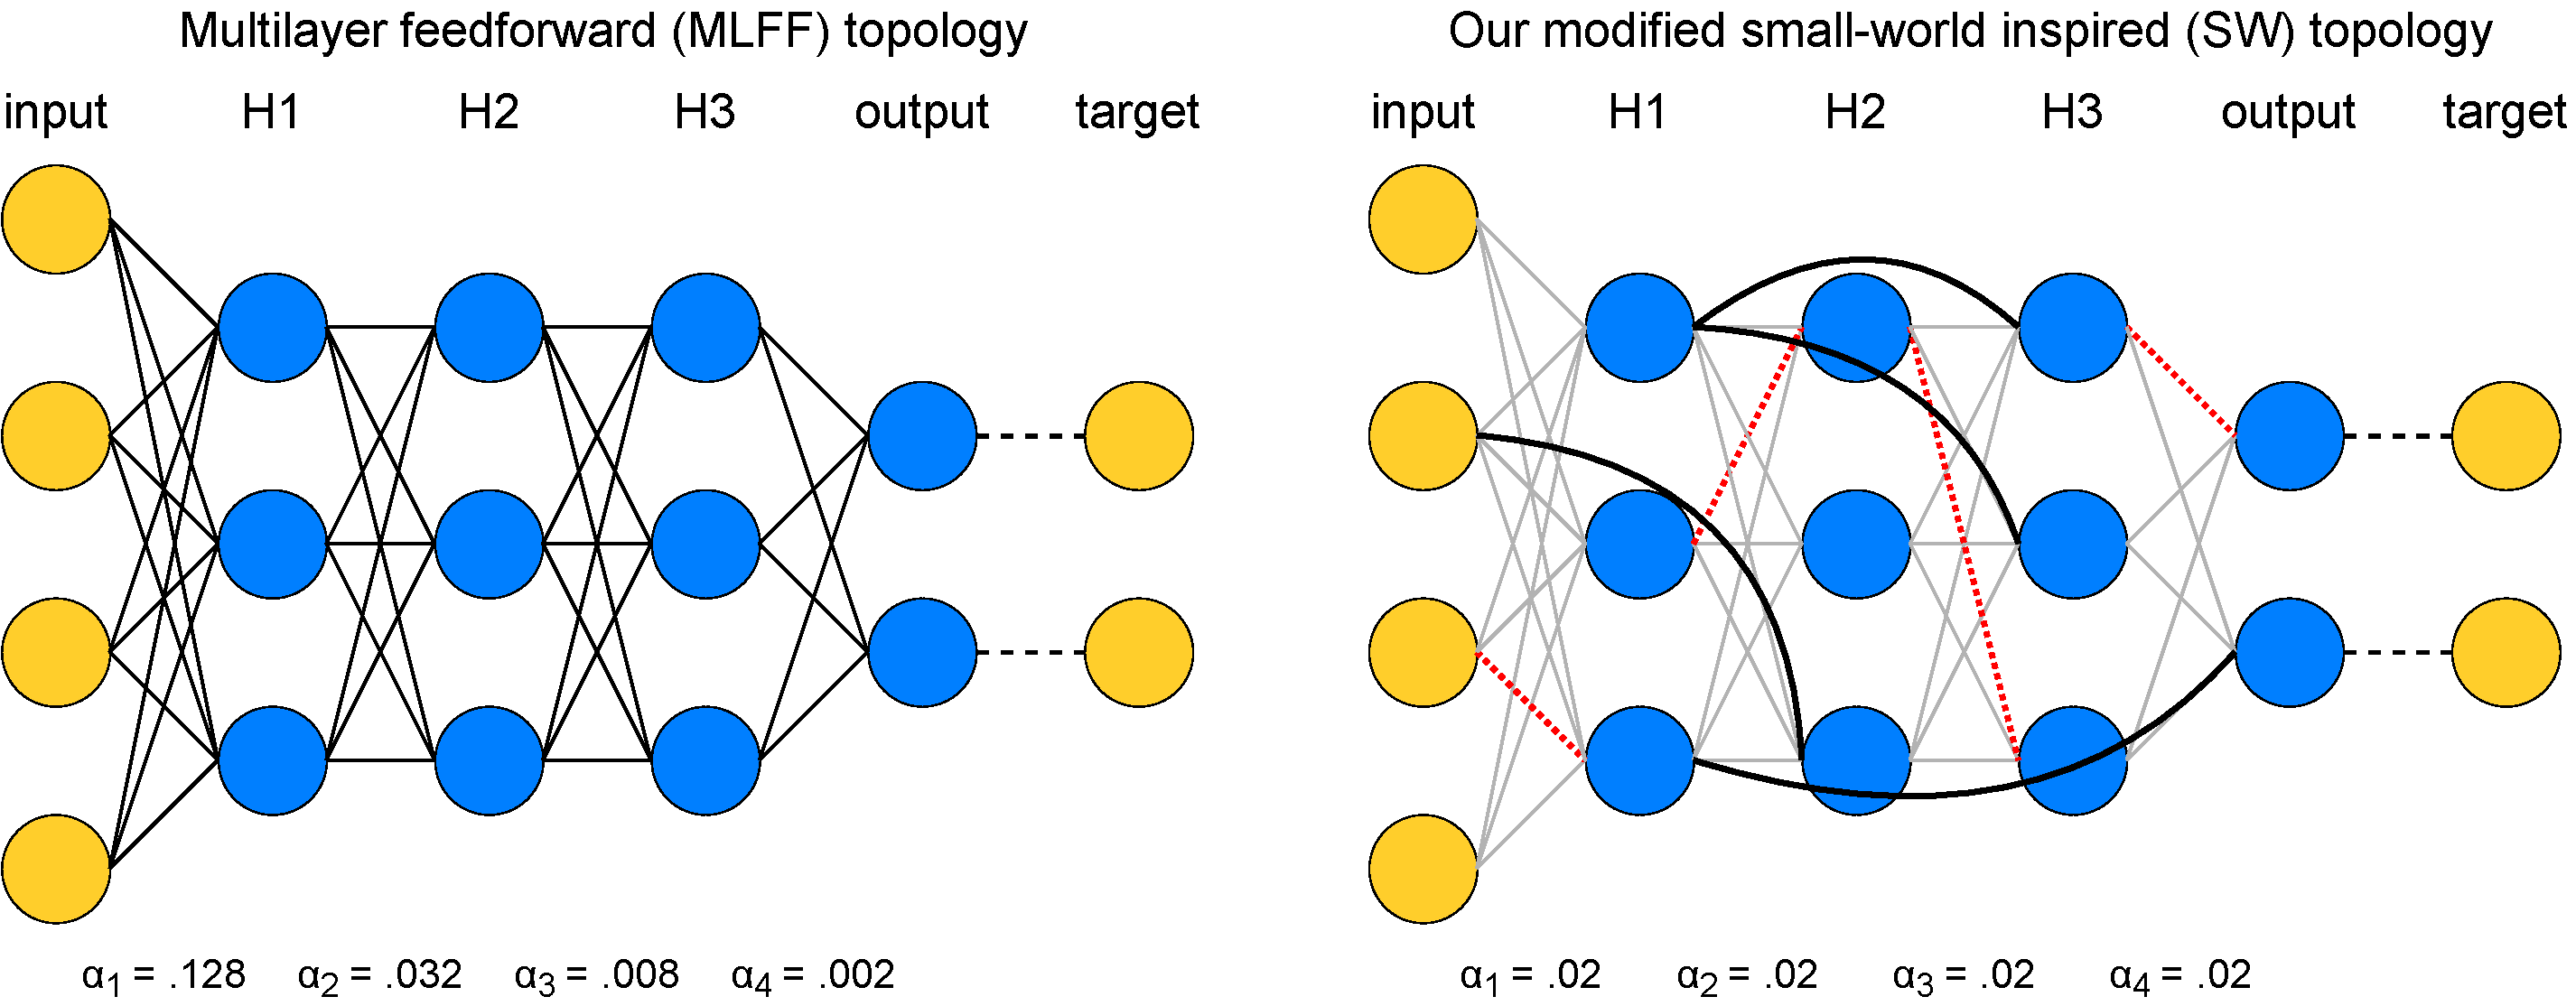
\includegraphics[width=6in]{figures/diagram.pdf}
	\caption{Illustration of our topological modifications to mitigate the vanishing gradient problem while using a global learning rate. (left) A network with MLFF topology as tested in \citep{scellier17}. Observe that the learning rate increases by a factor of 4 each time the distance from the output increases by one layer. (right) A network with SW topology, where a subset of connections have been replaced by random layer-skipping connections and per-layer learning rates have been replaced by a single global learning rate. Red dotted lines denote removed connections and solid black lines denote the layer-skipping connections replacing them.}
	\label{fig:diagram}
\end{figure}


\begin{algorithm}
\DontPrintSemicolon
\SetKwData{Network}{network}\SetKwData{PotConn}{potentialConns}\SetKwData{ExConn}{existingConns}\SetKwData{EC}{ec}\SetKwData{PC}{pc}
\SetKwData{ParamP}{p}\SetKwData{LoopP}{pp}
\SetKwInput{KwParam}{Parameter}
\KwIn{Network with MLFF topology to modify}
\KwParam{Probability \ParamP with which to replace a given preexisting connection}
\KwOut{Modified network with SW topology}
\BlankLine
\Network$\leftarrow\text{input network with MLFF topology}$\;
\PotConn$\leftarrow\{\text{pairs of distinct neurons in distinct layers that do not share a connection}\}$\;
\BlankLine
\For{existing connection \EC in \Network}{
\LoopP$\leftarrow$value drawn from uniform distribution $U[0, 1]$\;
\If{\LoopP $<$ \ParamP}{
remove connection \EC in \Network\;
randomly draw connection \PC from \PotConn\;
make connection \PC in \Network\;
remove \PC from \PotConn\;
add \EC to \PotConn\;
}
}
\caption{Algorithm to generate SW topology starting with a network with MLFF topology}\label{alg:ourtop}
\end{algorithm}

We generate a network with small-world inspired (SW) topology by first starting with a MLFF topology as described above in section \ref{sec:mlff_top}, then applying an algorithm similar to the one described in \citep{watts98} to randomly replace
\footnote{We have done a small number of trials in which layer skipping connections are added without removing an equal number of preexisting connections, and have observed behavior similar to that resulting from using algorithm \ref{alg:ourtop}.} existing connections by random layer-skipping connections with some probability $p$. This is done using algorithm \ref{alg:ourtop}, and the resulting SW topology is illustrated to the right in figure \ref{fig:diagram}. In all of our trials networks with SW topology are trained using a single global learning rate $\alpha$.

\section{Results}

\subsection{Evaluation on MNIST dataset}
\label{sec:origpaper}

Here we compare the behavior of networks with the SW topology presented here to those with the MLFF topology used in \citep{scellier17} when training on the MNIST dataset. We are using this dataset because it allows us to reproduce and extend the trials in \citep{scellier17}, and because it is non-trivial to effectively train on yet small enough to allow trials to complete in a reasonably-short amount of time.

\subsubsection{Classification error}\label{sec:network_performance}

\begin{figure}
	\centering
	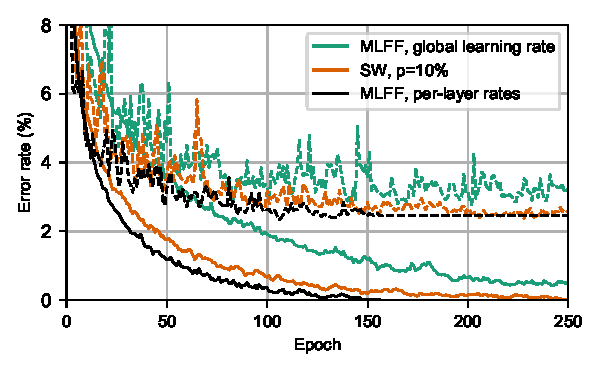
\includegraphics[width=4in]{figures/mnist_3layer_error.pdf}
	\caption{Performance on MNIST of networks with 3 500-neuron hidden layers. Dashed lines show the test error and solid lines show the training error. In black is a MLFF network with per-layer rates individually tuned to counter the vanishing gradient problem. In green is the same MLFF network but with a single global learning rate. In orange is a network with SW topology, $p=10\%$. Observe that the network with our topology trains almost as quickly as a network with per-layer rates, and significantly more-quickly than a network with a single learning rate.}
	\label{fig:error}
\end{figure}

Figure \ref{fig:error} shows the results of comparing the classification error on MNIST of a network with SW topology to that of a MLFF network with individually-tuned per-layer learning rates, as in \citep{scellier17}, and to that of a MLFF network with a single global learning rate. For all networks we use 3 500-neuron hidden layers, $\epsilon=.5$, $\beta=1.0$, 500 free-phase iterations, 8 weakly-clamped-phase iterations, and train for 250 epochs. For the SW network we use $p=10\%$ and a global learning rate $\alpha=.02$. For the MLFF network with per-layer rates we use learning rates $\alpha_1=.128$, $\alpha_2=.032$, $\alpha_3=.008$ and $\alpha_4=.002$. For the MLFF network with a single global learning rate, we use learning rate $\alpha=.02$.

We find that both the SW network and the MLFF network with per-layer rates significantly outperform the MLFF network with a single global learning rate during the first 250 epochs of training. The SW network achieves training and test error rates similar to those of the MLFF network with per-layer rates, albeit after around 100 additional epochs of training.

\subsubsection{Training rates of individual pairs of layers}\label{sec:rates}

\label{sec:mnist_perlayer}
\begin{figure}
	\centering
	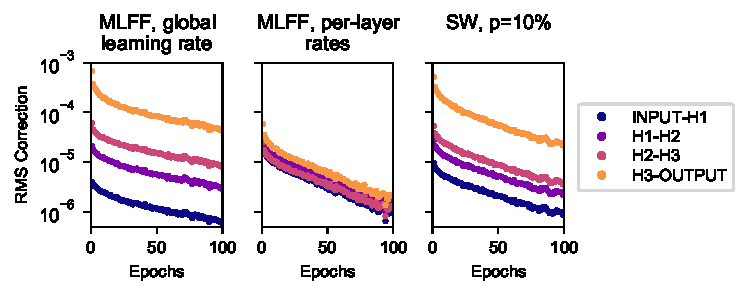
\includegraphics[width=4in]{figures/mnist_3layer_rates.pdf}
	\caption{Root mean square corrections to weights in different layers while training on MNIST, for networks with 3 500-neuron hidden layers. Measurements were taken after each batch, and averaged over each epoch. (left) A MLFF network with a single global learning rate. (center) A MLFF network with per-layer rates individually tuned to counter the vanishing gradient problem. (right) A network with SW topology, $p=10\%$. Observe that the correction magnitudes attenuate significantly with depth in the MLFF network with a single global learning rate, and that a network with SW topology reduces the severity of the issue, albeit less-effectively than individually tuning a learning rate for each layer.}
	\label{fig:rates}
\end{figure}

Here we consider the first 100 epochs of the trials described in section \ref{sec:network_performance} above and track the root-mean-square correction to weights connecting each pair of adjacent layers. Figure \ref{fig:rates} shows these values for the 3 network topologies, recorded after each batch and averaged over each epoch.

We can clearly see the vanishing gradient problem for the MLFF network with a single global learning rate (left), manifesting as attenuation with depth of the root-mean-square corrections to weights. The problem is addressed very-effectively by the use of manually-tuned per-layer learning rates (center), and is mitigated to a more-modest extent when we use SW topology with a global learning rate. It is noteworthy that the speed of training of these networks as shown in figure \ref{fig:error} is commensurate with the uniformity with which their layers train as shown in figure \ref{fig:rates}.

It can be seen that in the network with SW topology the weights connecting to the output layer train significantly faster than deeper weights, which cluster together; we have observed similar behavior in a variety of datasets and network dimensions. We suspect it has to do with the fact that output neurons connect directly to the target output, whereas because layer-skipping connections are not attached to the target output the other layers must connect indirectly through at least 2 connections.

\subsubsection{Behavior for varying $p$}\label{sec:sweep}

\begin{figure}
	\centering
	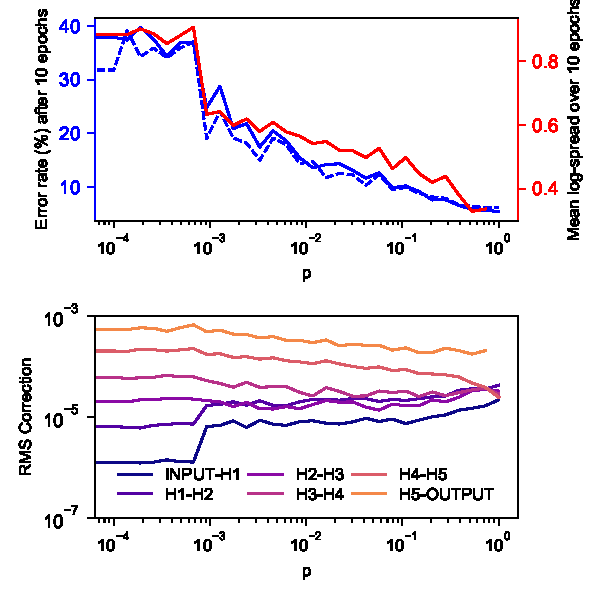
\includegraphics[width=4in]{figures/mnist_5layer_sweep.pdf}
	\caption{Behavior during the first 10 epochs of training on MNIST for a SW network with 5 100-neuron hidden layers for various values of $p$. (top) In solid and dashed blue are the training and test error rates after 10 epochs and in red is the log-spread (equation \ref{eqn:spread}) averaged over the 10 epochs. As expected, both values decrease as $p$ increases. There appears to be a strong linear correlation between the two, with coefficient of determination $r^2=.970$. This is consistent with our suspicion that mitigation of the vanishing gradient problem is the reason our topology tends to increase the rate at which layered networks train. (bottom) Root mean square corrections to weights in different layers, averaged over the 10 epochs. As expected, the spread of these values decreases as $p$ increases.}
	\label{fig:sweep}
\end{figure}

Figure \ref{fig:sweep} shows the behavior during the first 10 epochs of training on MNIST for a network with SW topology as $p$ is increased from 0 to .727. The network being tested has 5 100-neuron hidden layers and is trained with learning rate $\alpha=.015$, $\epsilon=.5$, $\beta=1.0$, 500 free-phase iterations and 8 weakly-clamped-phase iterations.

We see in the top graph that the training and test error rates after 10 epochs decay exponentially as $p$ increases. The bottom graph indicates that the RMS corrections to weights become more-uniform with depth as $p$ increases. Corrections to layers that do not connect directly to the output layer cluster closer together as $p$ increases, but it appears that the corrections to weights connecting directly to the output layer train faster than deeper weights with a gap that does not appear to decrease with $p$; this is similar to the behavior seen in section \ref{sec:rates}.

To quantify the spread of the RMS corrections as a single scalar, we introduce the statistic
\begin{equation}
\label{eqn:spread}
	\text{log-spread} = \text{Std. dev}\{\text{log}_{10}(w_l), l=1,\hdots,N+1\}
\end{equation}
where $N$ denotes the number of hidden layers in a network and $w_l$ denotes the root mean square magnitude of corrections to weights connecting the $l^{th}$ and $l+1^{th}$ layers from the input, averaged over all epochs of training. The $\text{log-spread}$ is plotted in the top graph alongside the error rate, and these values can be seen to have a strong linear correlation. The training error and the $\text{log-spread}$ have a coefficient of determination $r^2=.970$.


\subsubsection{Weight correction matrix}
\begin{figure}
	\centering
	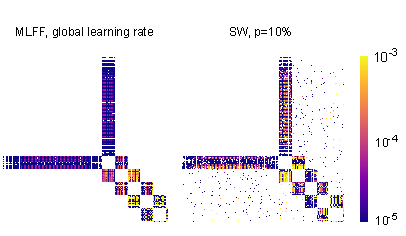
\includegraphics[width=4in]{figures/matrix_image.pdf}
	\caption{Mean absolute value correction matrix over 100 epochs for networks with 5 100-neuron hidden layers. A pixel at position $(i, j)$ corresponds to the magnitude of the correction to the connection weight between neurons $i$ and $j$. (left) A network with MLFF topology and a single global learning rate. (right) A network with SW topology, $p=10\%$. Observe that attenuation of these values with depth is less-significant in the latter than in the former.}
	\label{fig:matrices}
\end{figure}

In figure \ref{fig:matrices} we visualize the mean weight correction matrices resulting from training a MLFF network and a SW network with 5 100-neuron hidden layers as described in section \ref{sec:sweep}. Training on a batch yields a correction matrix $\mathbf{dW}$ where element $\mathbf{dW}_{ij}$ denotes the change to the connection weight between neurons $i$ and $j$; here we have recorded a matrix with element $(i, j)$ containing the average of $|\mathbf{dW}_{ij}|$ over 100 epochs of training and displayed it as an image with the color of a pixel at position $(i, j)$ encoding the magnitude of $|\mathbf{dW}_{ij}|$ as indicated by the legend.

As expected, there is attenuation with depth to weight correction magnitudes in a MLFF network with a single global learning rate, and transitioning to a network with SW topology reduces the severity of the problem. An interesting feature of the SW matrix that is visible upon close inspection is that layer-skipping connections tend to receive larger correction magnitudes when they are closer to the output of the network. Striations can be seen in correction magnitudes, which we believe correspond to sections of images in the MNIST dataset that contain varying amounts of information; for example, for corrections connecting to the input layer, there are 28 striations which likely correspond to the 28 rows of pixels in an image of a digit, with pixels closer to the edges of the images typically blank and pixels closer to the centers of the images typically containing most of the variation that encodes a digit.

\subsection{Evaluation on various datasets and topologies}
\label{sec:comparison}

Here we evaluate the presence of the vanishing gradient problem and the effectiveness of our topology at addressing it on MNIST \citep{mnist1998}, Fashion MNIST (FMNIST) \citep{fmnist2017}, and the diabetes and wine toy datasets distributed in scikit-learn \citep{sklearn2011} with various network architectures. Our results are shown in table \ref{tbl:results}. For all of these trials we use $\beta=1.0$ and $\epsilon=.5$.

We report the training and test error after 100 epochs, as well as the log-spread (equation \ref{eqn:spread}). We see that networks with SW topology, $p=10\%$, have a consistently smaller log-spread than networks with a MLFF topology and a single global learning rate. This is typically associated with smaller error rates, although in some circumstances the error rates do not change significantly. We have observed that all of these networks behave in ways that are qualitatively similar to the networks explored in section \ref{sec:origpaper}.

\begin{table}
\centering
\resizebox{\columnwidth}{!}{
\begin{tabular}{|c|c|c|c|c|c|c|c|c|}
\hline
 Dataset & Layer sizes & Topology & L.R. & Iterations &Error (train/test)  & log-spread \\\hline
 Diabetes & 10-10-10-10-10-10-1 & MLFF & .01 & 1000/12 & .00698/.00876 & 1.291 \\
 Diabetes & 10-10-10-10-10-10-1 & SW, p=10\% & .01 & 1000/12 & .00704/.00760 & \textbf{.629} \\
 Diabetes & 10-10-10-10-10-10-10-10-10-1 & MLFF & .01 & 5000/18 & -/- & - \\
 Diabetes & 10-10-10-10-10-10-10-10-10-1 & SW, p=10\% & .01 & 5000/18 & -/- & \textbf{-} \\
 Wine & 13-10-10-10-10-10-3 & MLFF & - & 1000/12 & -/- & - \\
 Wine & 13-10-10-10-10-10-3 & SW, p=10\% & - & 1000/12 & -/- & - \\
 Wine & 13-5-5-5-5-5-5-5-5-5-5-3 & MLFF & - & 5000/22 & -/- & - \\
 Wine & 13-5-5-5-5-5-5-5-5-5-5-3 & SW, p=10\% & - & 5000/22 & -/- & - \\
 MNIST & 784-500-500-500-10 & MLFF & .02 & 500/8 & .0170/.0310 & .689 \\
 MNIST & 784-500-500-500-10 & SW, p=10\% & .02 & 500/8 & .00675/.0272 & \textbf{.545} \\
 MNIST & 784-100-100-100-100-100-10 & MLFF & .015 & 1000/12 & .156/.131 & .867 \\
 MNIST & 784-100-100-100-100-100-10 & SW, p=10\% & .015 & 1000/12 & .0407/.0540 & \textbf{.450} \\
 FMNIST & 784-100-100-100-100-100-10 & MLFF & .015 & 1000/12 & .266/.255 & .862 \\
 FMNIST & 784-100-100-100-100-100-10 & SW, p=10\% & .015 & 1000/12 & .152/.164 & \textbf{.484} \\\hline
\end{tabular}
}
\caption{Comparison of MLFF and SW topologies with various datasets and network architectures. In all tests networks were trained for 100 epochs. Observe that the vanishing gradient problem, quantified by the log-spread (equation \ref{eqn:spread}), is consistently less-severe when using the SW topology over the MLFF topology.}
\label{tbl:results}
\end{table}


\section{Directions for Future Research}

There are several directions in which future research could be taken:
\begin{itemize} 
\item Evaluating the effectiveness of this approach on hard datasets, such as CIFAR and ImageNet.
\item Evaluating the effect of $p$ on a network's test error in the long term.
\item Exploring the effectiveness of a network when layer-skipping connections are used during training and removed afterwards.
\item Devise and mathematically justify a weight initialization scheme for layer-skipping connections.
\item Mathematically justify the empirical results we have seen when using SW topology.
\end{itemize}

\section*{Conflict of Interest Statement}

The authors declare that the research was conducted in the absence of any commercial or financial relationships that could be construed as a potential conflict of interest.

The U.S. Government is authorized to reproduce and distribute reprints for governmental purposes notwithstanding any copyright annotation thereon.
%
%\section*{Author Contributions}
%
%The Author Contributions section is mandatory for all articles, including articles by sole authors. If an appropriate statement is not provided on submission, a standard one will be inserted during the production process. The Author Contributions statement must describe the contributions of individual authors referred to by their initials and, in doing so, all authors agree to be accountable for the content of the work. Please see  \href{http://home.frontiersin.org/about/author-guidelines#AuthorandContributors}{here} for full authorship criteria.
%
%\section*{Acknowledgments}
%This is a short text to acknowledge the contributions of specific colleagues, institutions, or agencies that aided the efforts of the authors.
%
\bibliographystyle{frontiersinSCNS_ENG_HUMS}

\bibliography{references.bib}

\clearpage
\begin{appendices}




%\begin{figure}[h!]
%\begin{center}
%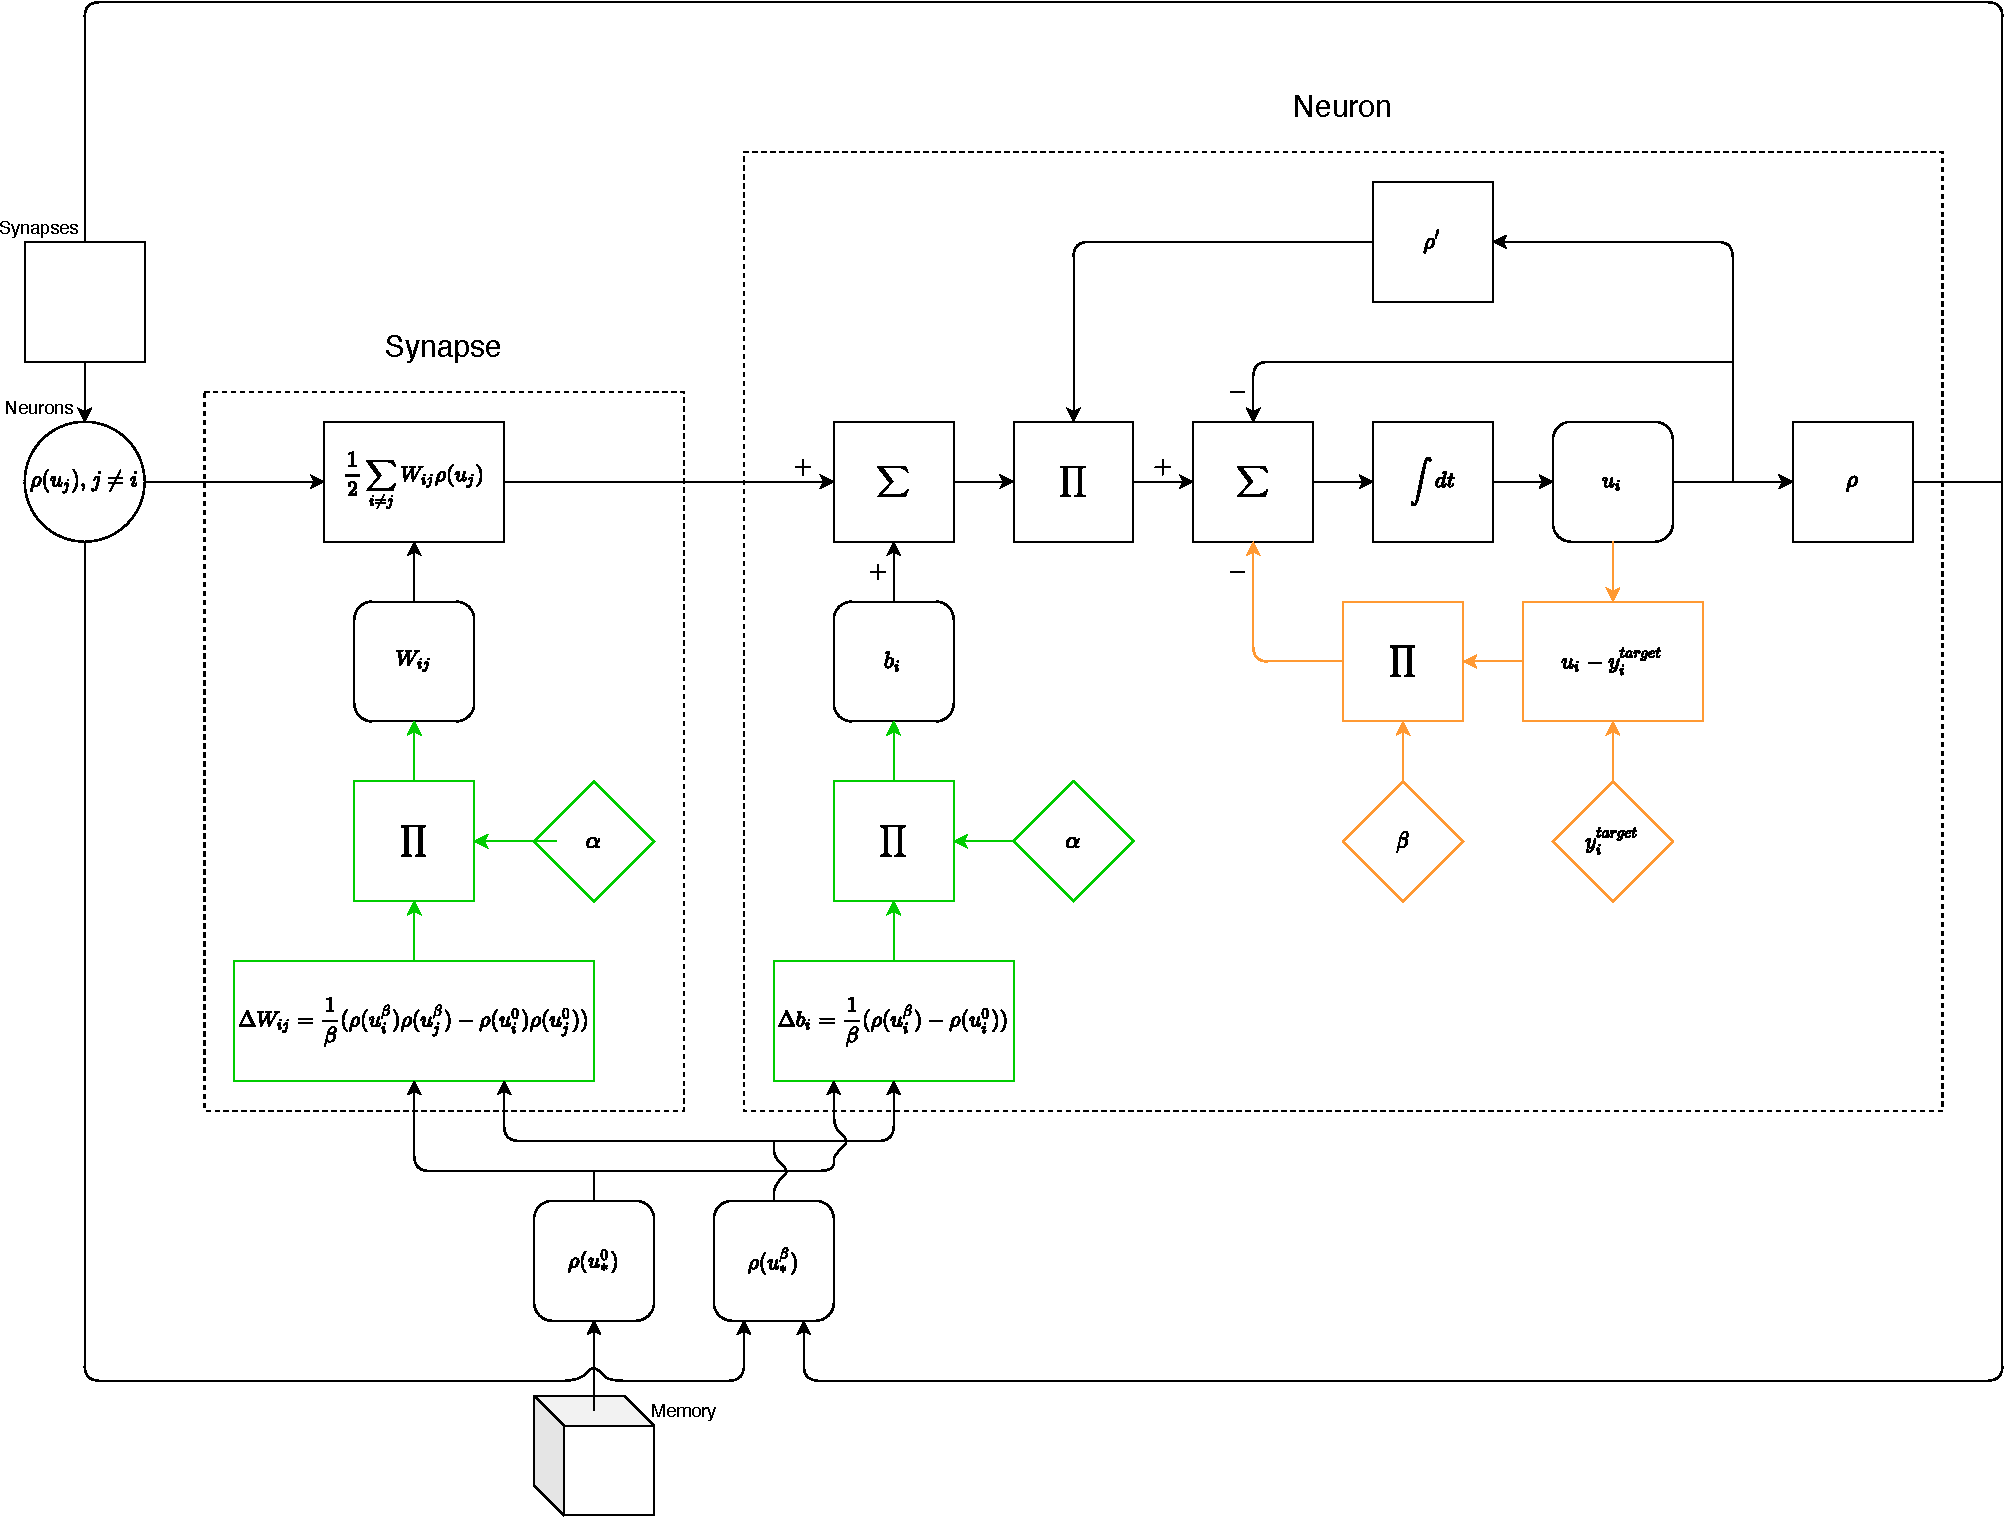
\includegraphics[width=\textwidth]{figures/eqp_bd.pdf}
%\end{center}
%\caption{Illustration of the functionality needed to implement equilibrium propagation in hardware. Black lines denote functionality needed in the free phase. Green lines denote functionality to correct parameters. Orange lines denote functionality needed only by output neurons, that is unique to the weakly-clamped phase. There is no functionality unique to the weakly-clamped phase that is needed by all neurons.} \label{fig:eqp_bd}
%\end{figure}
%\begin{figure}[h!]
%\begin{center}
%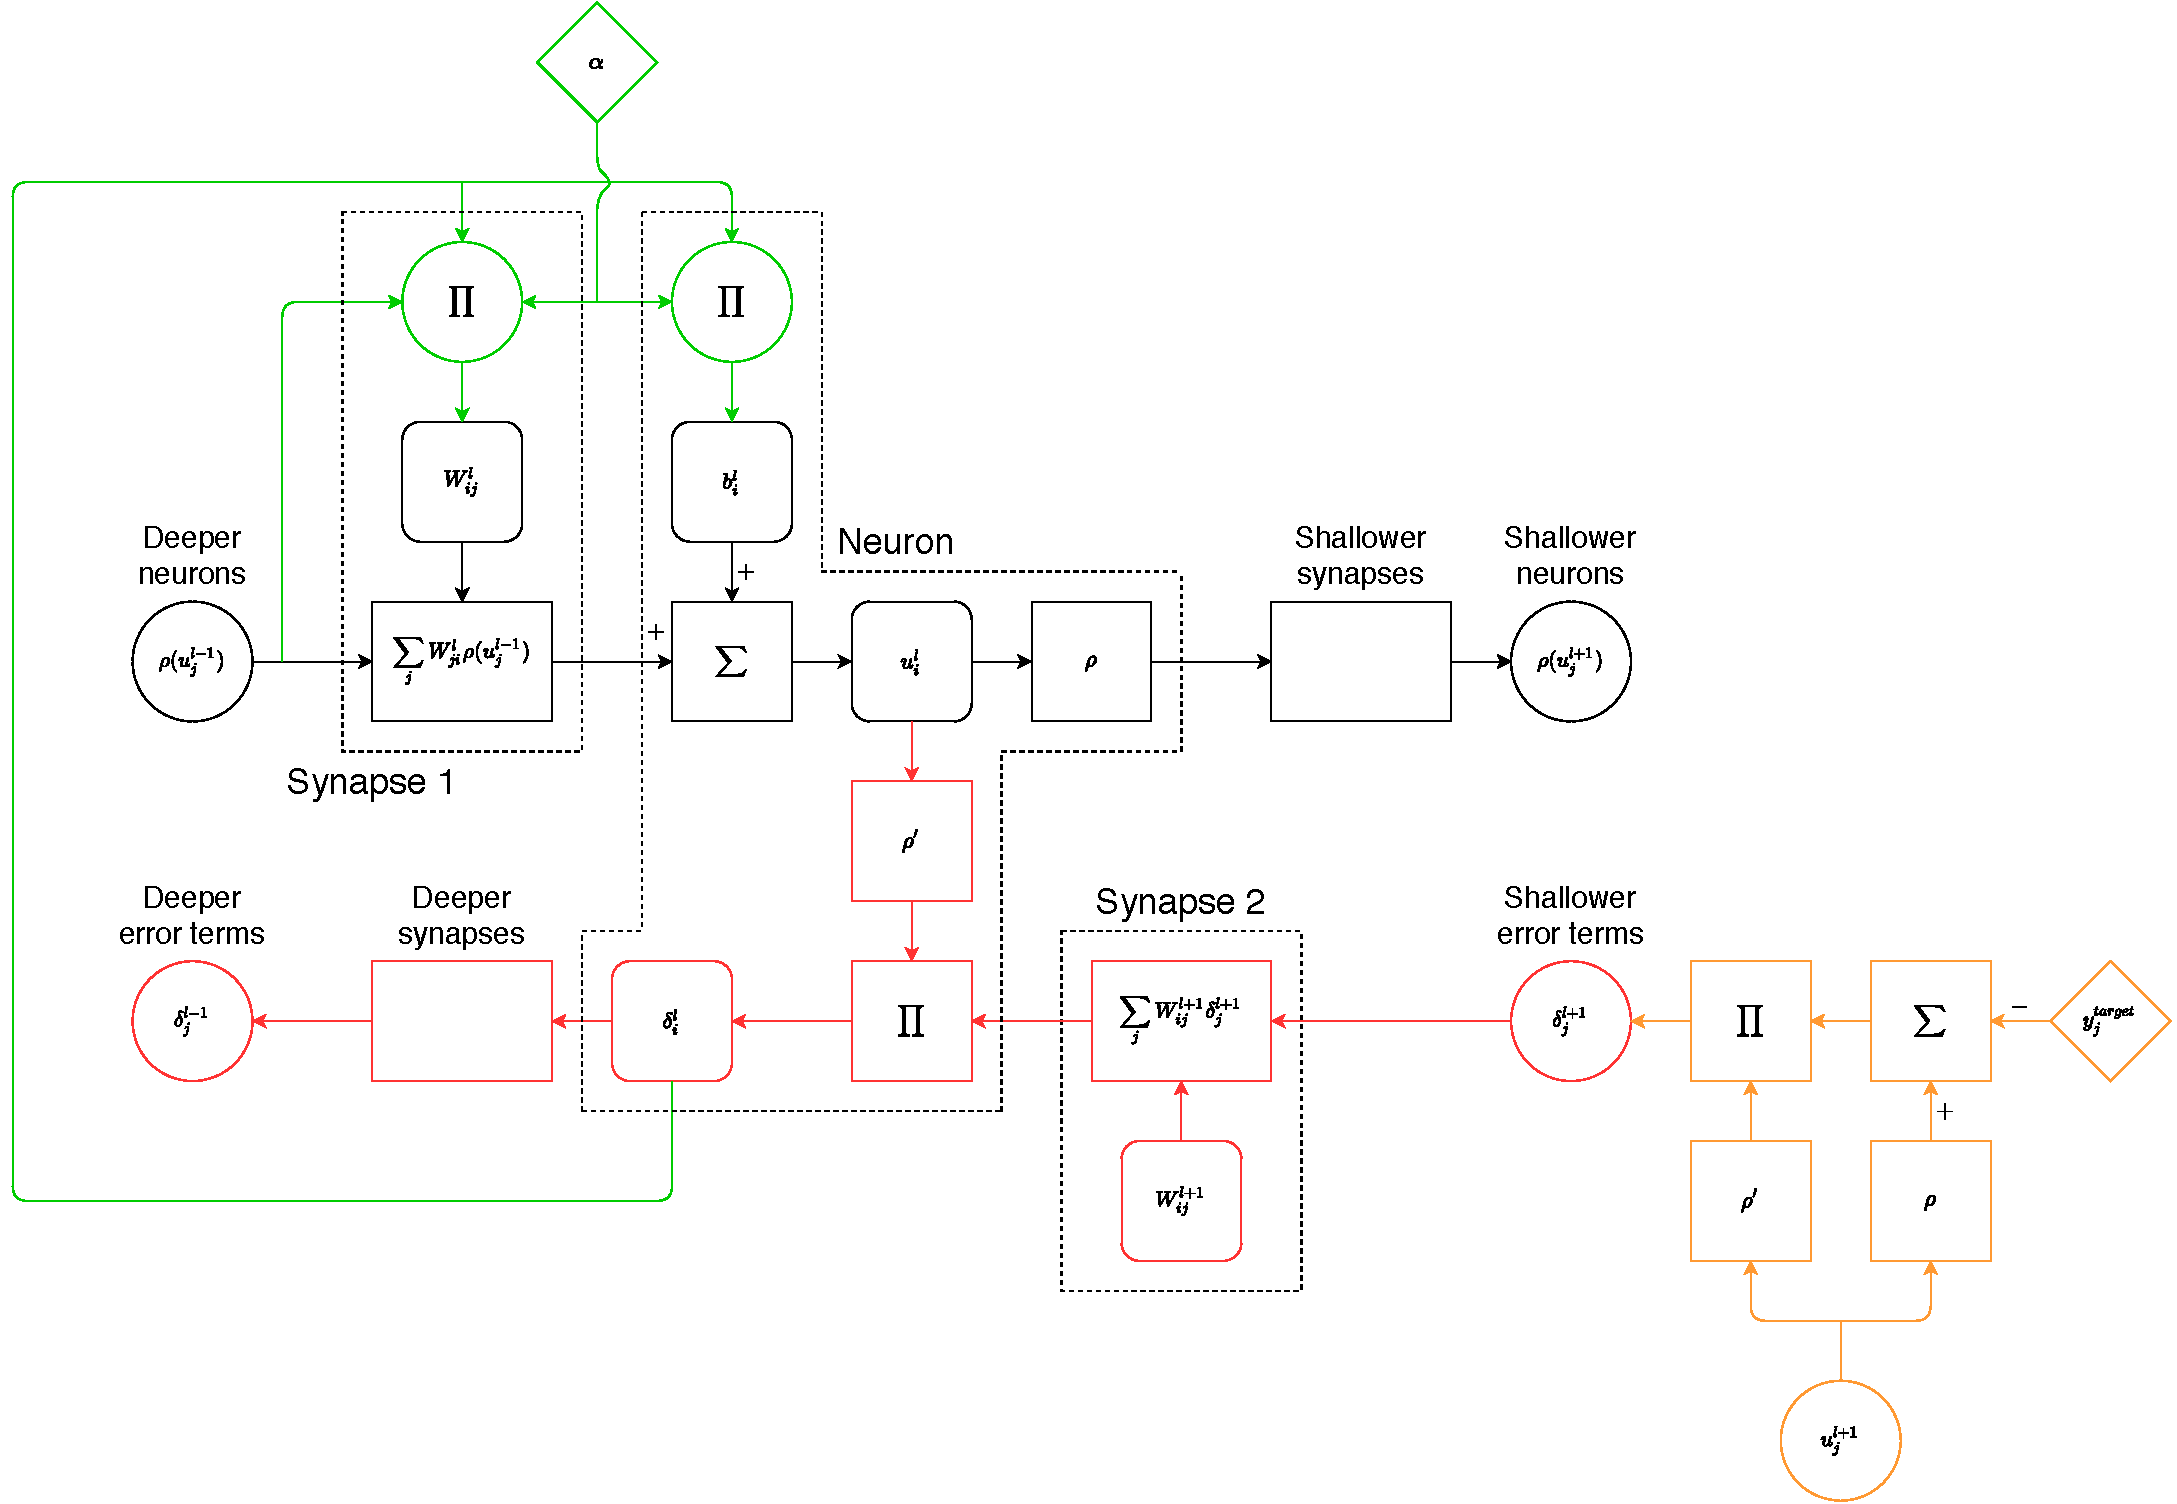
\includegraphics[width=\textwidth]{figures/backprop_bd.pdf}
%\end{center}
%\caption{Illustration of the functionality needed to implement backpropagation in hardware. Black lines denote functionality needed in the forwards phase. Green lines denote functionality to correct parameters. Red lines denote functionality unique to the backwards phase that is needed by all neurons. Orange lines denote functionality needed only by output neurons, that is unique to the backwards phase.} \label{fig:backprop_bd}
%\end{figure}
\clearpage
\section*{Tables}
\begin{table}[h!]
\begin{center}
\begin{tabular}{|L||L|L|}
\hline
&Backpropagation & Equilibrium Propagation \\ \hline\hline
Number of distinct computations & 2 -- computations during forwards and backwards phases are distinct & $\approx 1$ -- hidden neurons perform same computation in both phases. Output neurons perform a similar but modified version of the same computation. \\ \hline
Types of connections & Unidirectional to transmit activation to shallower neighbors and error to deeper neighbors & Bidirectional to each neighbor \\ \hline
Memory & Space to store activation and error term for each neuron & Space to store free and weakly-clamped activations for each neuron \\ \hline
Order of computations & Forwards propagation phase where layers are computed from deepest to shallowest; backwards propagation phase where layers are computed from shallowest to deepest; parameter update phase & Free phase where all neurons evolve simultaneously; weakly-clamped phase where all neurons evolve simultaneously; parameter update phase \\ \hline
Nonlinear activation function & Yes & Yes \\ \hline
Derivative of nonlinear activation function & Yes & Yes \\ \hline
Correction computation & Corrections require dedicated circuitry unique from that implementing propagation & Corrections require dedicated circuitry unique from that implementing evolution \\ \hline
\end{tabular}
\end{center}
\caption{Comparison of the capabilities a hardware neuron would need in order to implement backpropagation and equilibrium propagation.} \label{table:bp_eqp_contrast}
\end{table}

\section{Comparing the computational complexity of equilibrium propagation and backpropagation}
\label{sec:comparison}
The main motivations for using equilibrium propagation instead of an alternative 
machine learning technique (such as deep learning using backpropagation for training) are 1) to 
gain insight into the operation of the brain by developing target-based learning approaches in 
biologically plausible networks and 2) to develop algorithms that are more easily implemented in 
hardware. Below we qualitatively compare the hardware that would be needed for implementation of 
equilibrium propagation versus for backpropagation on a standard feedforward network to gain 
insight into the utility of these networks.

\subsection{Requirements of equilibrium propagation}


\begin{figure}
\begin{center}
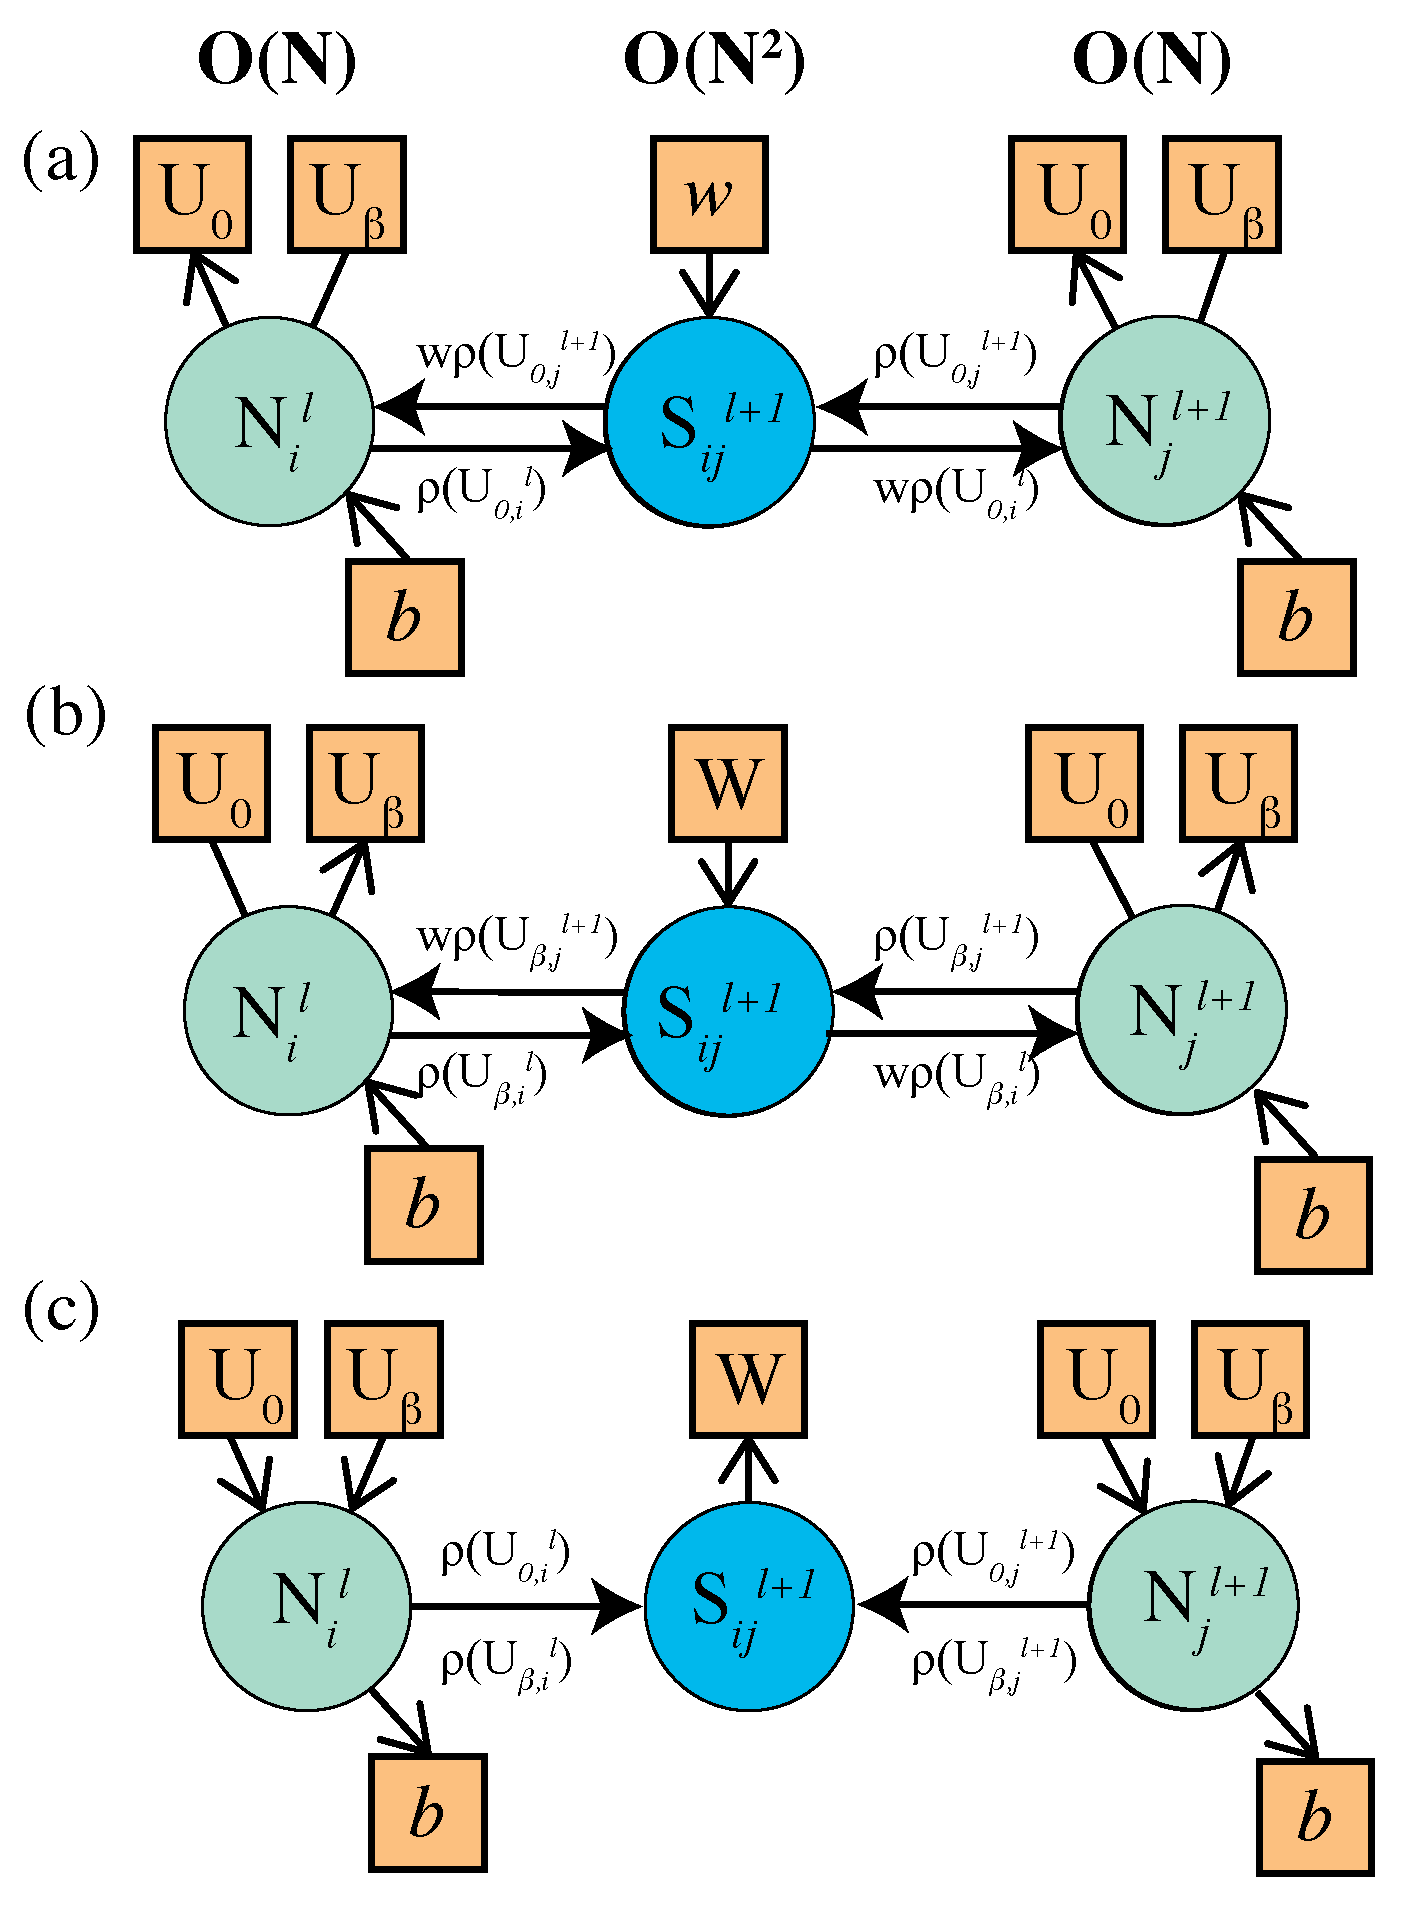
\includegraphics[width=10cm]{figures/eq_prop_sb.pdf}
\end{center}
\caption{Illustration of the functionality needed to implement equilibrium propagation in hardware. Yellow squares indicate a value that must be stored in memory for a subsequent phase. The circles indicate ($N$) neuron and ($S$) synapse devices with the associated functions described in the text. (a) The functionality required by the neurons and synapses in the free running phase. (b) The functionality of the neurons and synapses (except output neurons) in the weakly clamped phase. (c) The functionality of the neurons and synapses in the weight and bias update phase.} \label{fig:eq_prop}
\end{figure}

Just as in the algorithm, to implement equilibrium propagation in hardware, three
different phases of hardware operation are required. In the first (free) phase, it follows
from equations \ref{eqn:energy}, \ref{eqn:total_energy} and \ref{eqn:dynamics} that to determine 
its state, the $i$-th neuron in a network must compute $$\frac{\partial F}{\partial 
u_i}=u_i-\frac{1}{2}\rho'(u_i)[\sum_{i\neq j}W_{ij}\rho(u_j)+b_i],$$ plus the term 
$\beta(u_i-y_i^{target})$ for output neurons when using a squared-error cost function, and then 
integrate the result over time. Parameter correction rules are given by equations 
\ref{eqn:weight_correction} and \ref{eqn:bias_correction}. This is exactly the 
operation of an analog leaky integrate and fire neuron, as for example implemented in the 
neuromorphic hardware platforms of references \citep{indiveri2011, schemmel2010} among others. A 
qualitative diagram of potential neuron and synapse devices and their output and read/write to 
memory operations are shown in the diagram in figure \ref{fig:eq_prop} (a). At each neuron $N^l_{i}$ 
the value of $U^{l+1}_{i,0}$ is written to memory and the nonlinear function $\rho$ is applied 
before sending to the synapse device, where it is multiplied by the weight $w^{l+1}_{ij}$ which is 
read from memory by the synapse device. These weighted outputs are summed at the input of the next 
neuron device ($N^{l+1}_j$) and added to a bias value $b^{l+1}_j$ that is read from memory to 
generate $U_{l+1}$.

In the second (weakly-clamped) phase, shown in figure \ref{fig:eq_prop} (b), the operation of the 
hardware is exactly the same as in (a), with the value $U_{\beta}$ written to memory at each 
neuron. Not shown in figure \ref{fig:eq_prop} is the functionality at the output neurons which are 
weakly clamped and have a new function in this phase.

Finally, in the third phase, the weights and biases are updated as shown in figure \ref{fig:eq_prop} (c). At each neuron device the values of $U_0$ and $U_\beta$ are read from memory and $\rho({U_0})$ and $\rho({U_\beta})$ are calculated. At the synapse device, the computation of equation \ref{eqn:weight_correction} is performed using these values from the pre- and post- synaptic neurons to calculate the weight update $\Delta w$, and the value of the weight in memory is updated to $w+\alpha\Delta w$.  Similar updates are applied to the bias $b$ at every neuron according to equation \ref{eqn:bias_correction}. As shown at the top of  \ref{fig:eq_prop}, for $N$ such neurons per layer, there will be $N^2$ synapses.

%%A block diagram of this process is shown in figure \ref{fig:eqp_bd} and qualitatively describes 
%%one way equilibrium propagation could potentially be implemented in hardware.

\subsection{Requirements of backpropagation}

\begin{figure}
\begin{center}
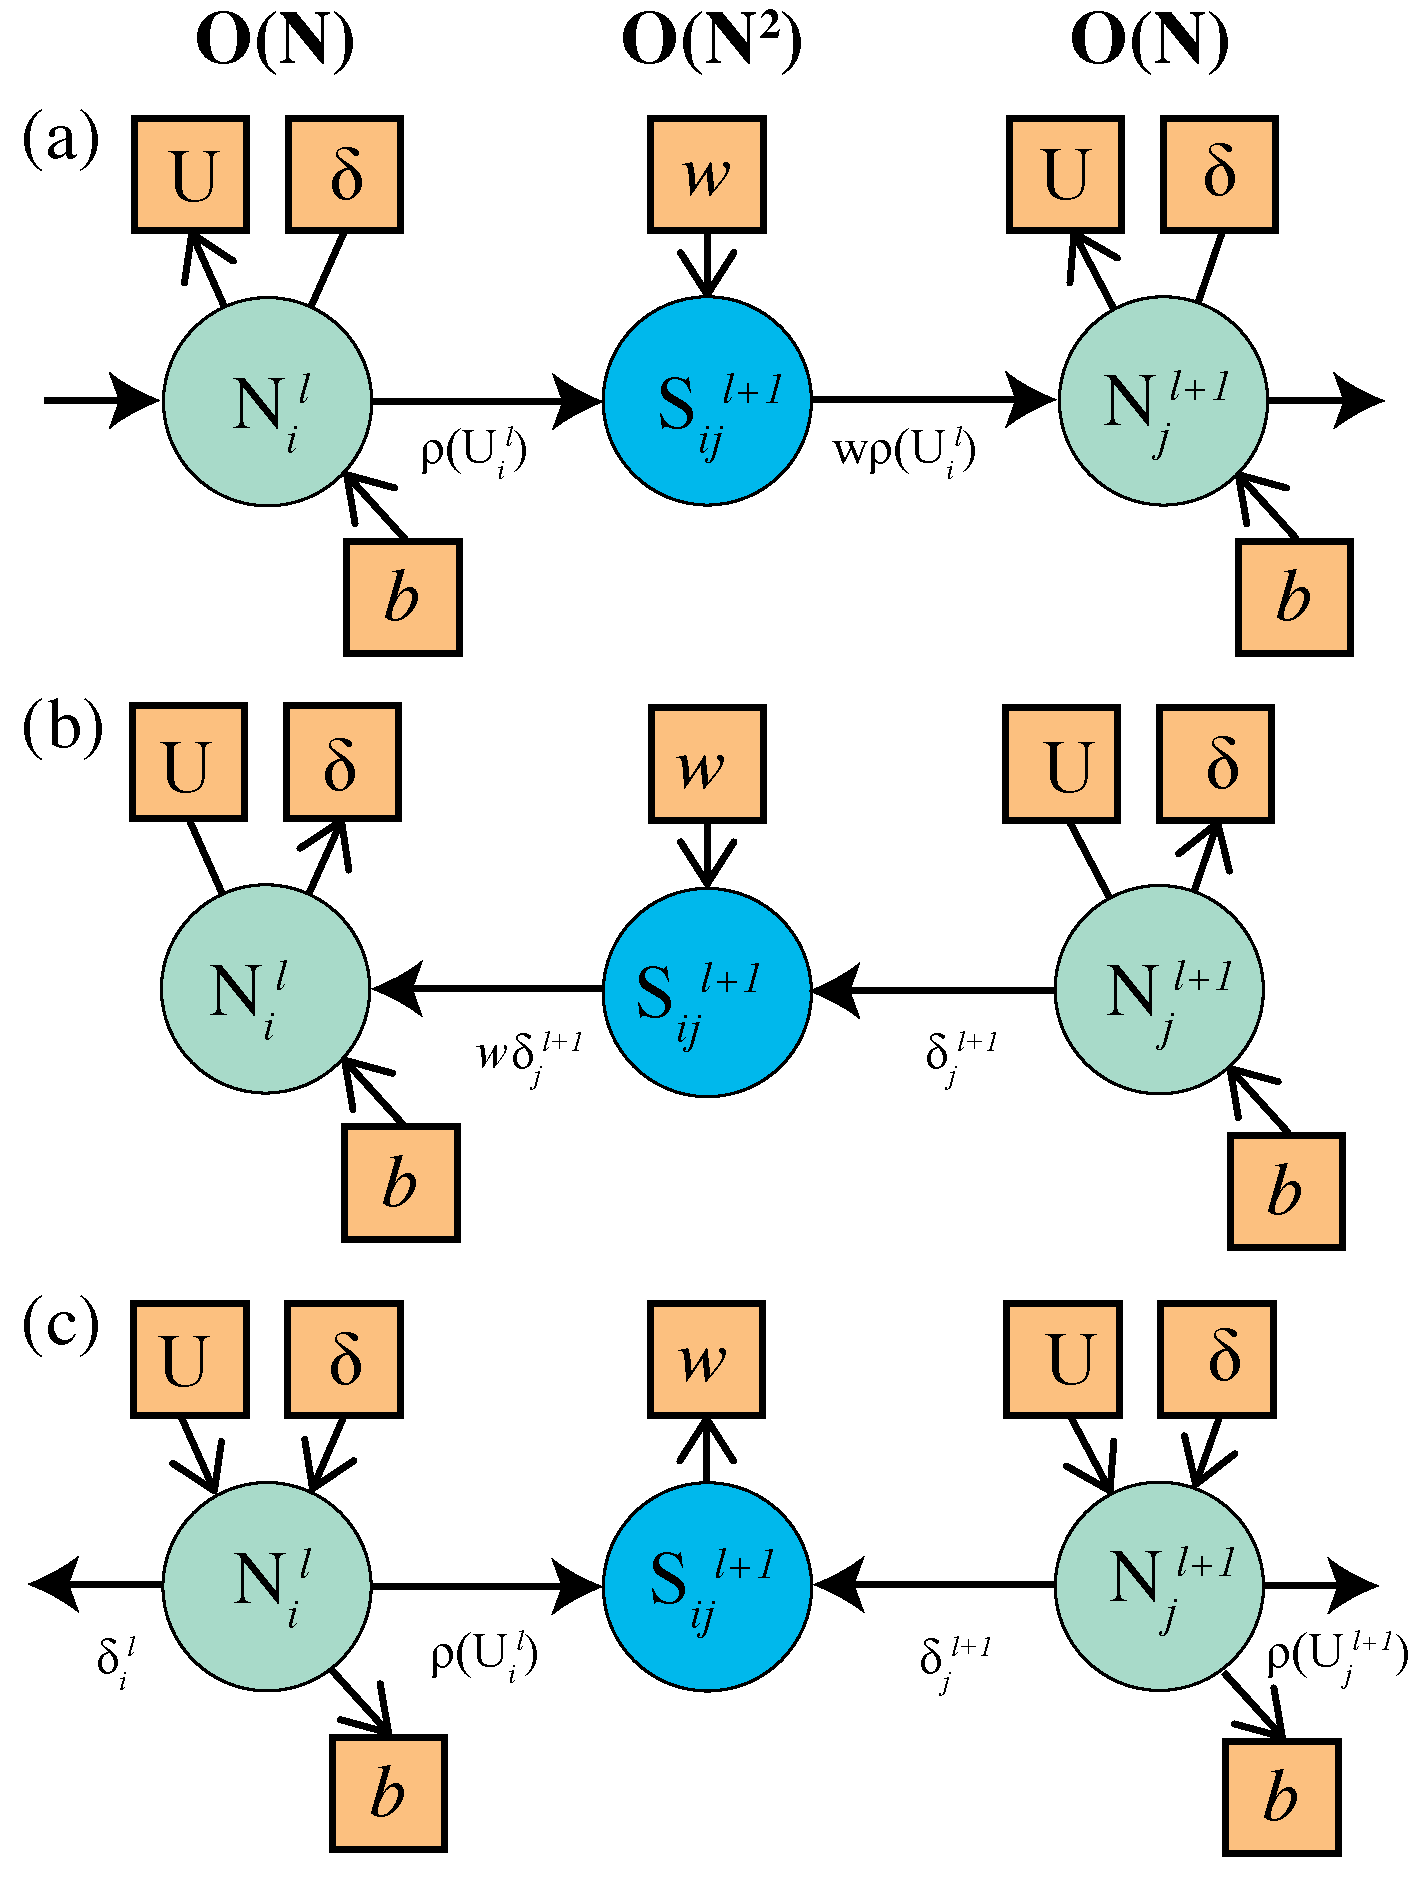
\includegraphics[width=10cm]{figures/back_prop_sb.pdf}
\end{center}
\caption{Illustration of the functionality needed to implement backpropagation in hardware. Yellow squares indicate a value that must be stored in memory for a subsequent phase. The circles indicate ($N$) neuron and ($S$) synapse devices with the associated functions described in the text. (a) The functionality required by the neurons and synapses in the forward pass phase. (b) The functionality of the neurons and synapses (except the last layer of neurons) in the backpropagation phase. (c) The functionality of the neurons and synapses in the weight and bias update phase.} \label{fig:back_prop}
\end{figure}

Backpropagation is an algorithm for training networks using gradient descent. It is 
most typically applied to feedforward neural networks, in which the activation value of a neuron 
$i$ in layer $l$ is given by $$\rho(u_i^l)=\rho(\sum_jW_{ij}^lu_j^{l-1}+b_i^l).$$ This
is very similar to the free running situation in equilibrium propagation, with the main difference 
being that the connections are unidirectional. The qualitative implementation of this inference
phase in hardware is shown in Fig. \ref{fig:back_prop} (a). Using backpropagation, the 
parameters are then updated by computing error
correction terms $\delta_i^l$ for each neuron $i$ in layer $l$; for the output layer $L$ the 
correction is $$\delta_i^L=\rho'(u_i^L)(\rho(u_i^L)-y_i^{target})$$ and for deeper layers it is
$$\delta_i^l=\rho'(u_i^l)\sum_jW_{ij}^{l+1}\delta_j^{l+1}.$$ The implementation of 
this in hardware is shown in figure \ref{fig:back_prop} (b) (excluding layer $L$). Note that the data
is now moving in the opposite (backwards) direction, and unlike in the case of equilibrium 
propagation, the functions implemented by the neurons are entirely different to the operation in 
the forward phase shown in (a). In a final phase, weights are corrected using $$\Delta 
W_{ij}^l=\rho(u_i^{l-1})\delta_j^l$$ and biases using 
$$\Delta b_i^l=\delta_i^l.$$ This is shown in figure \ref{fig:back_prop} (c).

%%The block diagram in figure \ref{fig:back_prop} qualitatively describes a way this algorithm 
%%could potentially be implemented in hardware. 

\subsection{Comparison}

The most-significant difference between the algorithms is that in equilibrium propagation, the free
and weakly-clamped phases of training are identical for most neurons and the weakly-clamped phase 
requires only slight modification to output neurons, whereas in backpropagation these phases demand significantly-different functionality from essentially all neurons. There are two other differences that we do not believe to be significant in terms of ease of implementation in hardware. One is that in equilibrium propagation each pair of neurons is joined by a bidirectional synapse, whereas in backpropagation each pair is joined by two unidirectional synapses; we expect both cases to be equally easy to implement. The other is that in equilibrium propagation, each neuron must remember its equilibrium state after the free phase while it executes the weakly-clamped phase; since backpropagation implies a state variable for the activation and error term of each neuron, the memory requirement of each neuron should be the same in both cases.
For a hardware implementation, the need for distinct free and weakly-clamped phases (temporally non-local credit assignment) significantly reduces the advantages associated with the spatially local credit assignment. Recently there has been new work that indicates that the algorithm can be modified to eliminate the need for both phases \citep{ernoult2020}. This would significantly reduce the memory requirements of the algorithm. Various characteristics of both algorithms are compared side-by-side in table \ref{table:bp_eqp_contrast}. 

\end{appendices}

\clearpage
\section*{Figures}

%\begin{figure}[h!]
%\begin{center}
%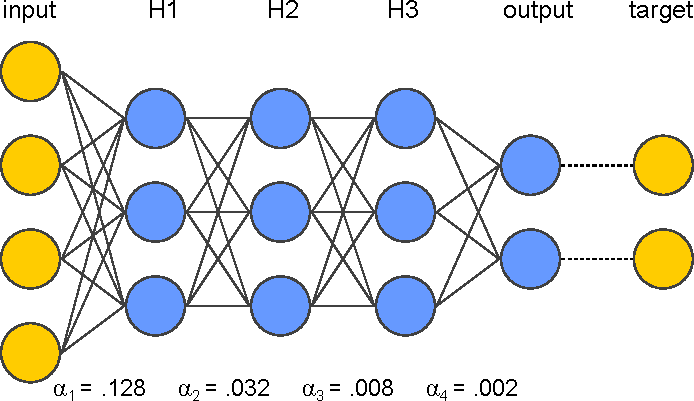
\includegraphics[width=\textwidth]{figures/topology1_basic.pdf}
%\end{center}
%\caption{Topology of the layered network tested in \citep{scellier17}. All pairs of neurons in adjacent layers are connected. All connections are bidirectional. To compensate for the vanishing gradient problem, the learning rate $\alpha$ is reduced by a factor of 4 each time distance from the output decreases by one layer.} \label{fig:top_basic}
%\end{figure}
%\begin{figure}[h!]
%\begin{center}
%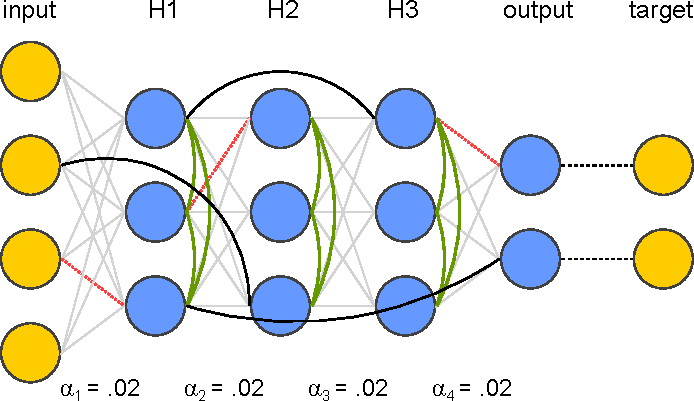
\includegraphics[width=\textwidth]{figures/topology2_modified.pdf}
%\end{center}
%\caption{Our modifications to the topology of figure \ref{fig:top_basic} to avoid a vanishing gradient while using a global learning rate. Red dotted lines denote connections that have been removed, black lines denote their replacements, and green solid lines denote added intralayer connections. All connections are bidirectional.} \label{fig:top_sw}
%\end{figure}
%\begin{figure}[h!]
%\begin{center}
%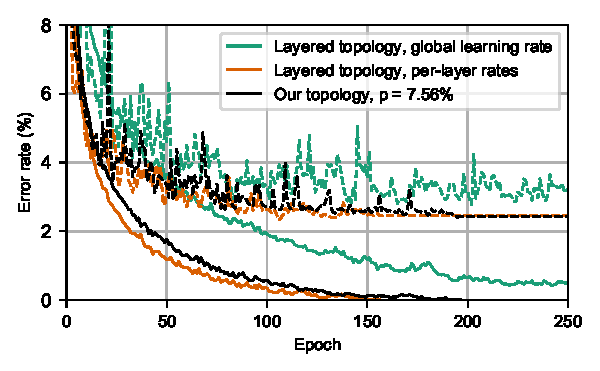
\includegraphics[width=\textwidth]{figures/MNIST_network_comparison.pdf}
%\end{center}
%\caption{Performance on MNIST of the networks in section \ref{sec:implementation}. Dashed lines show the test error and solid lines show the training error. In green is a layered network with a global learning rate (section \ref{sec:basic_topology_uniform}), in orange is a layered network with per-layer rates individually tuned to counter the vanishing gradient problem (section \ref{sec:basic_topology}), and in green is a network with our topology, $p=7.56\%$ (section \ref{sec:our_topology}). Observe that our topology is almost as effective as per-layer rates at countering the vanishing gradient problem that impedes training of the layered network with a global learning rate.} \label{fig:mnist_comparison}
%\end{figure}
%\begin{figure}[h!]
%\begin{center}
%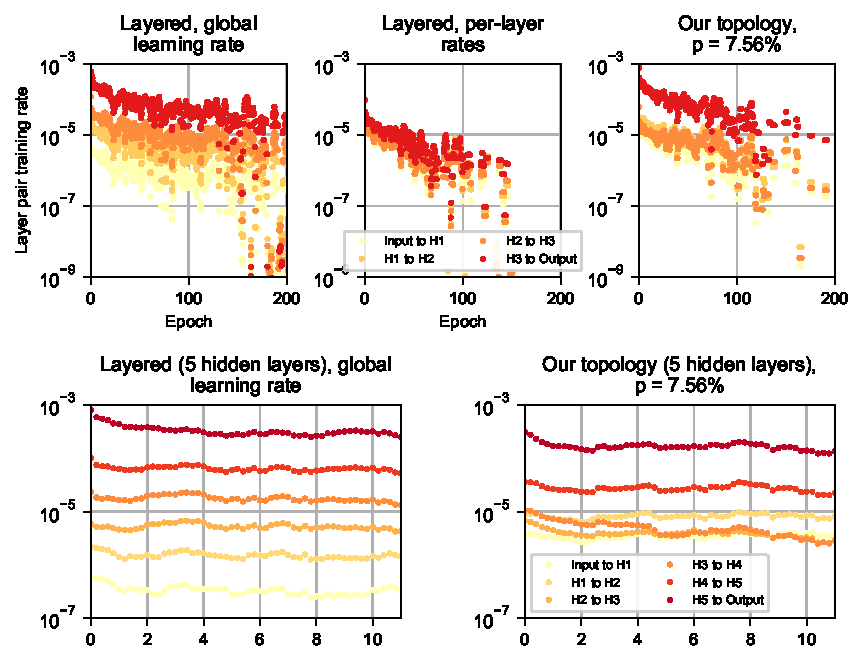
\includegraphics[width=\textwidth]{figures/MNIST_individual_layers.pdf}
%\end{center}
%\caption{Root-mean-square corrections to weights in different layers while training on MNIST, for the networks in section \ref{sec:implementation}. For clarity, values were subjected to an 11-point centered moving average. (left) A layered network with a single global learning rate (section \ref{sec:basic_topology_uniform}). (center) A layered network a unique, individually-tuned learning rate for each layer (section \ref{sec:basic_topology}).  (right) A network with our topology, $p = 7.56\%$ (section \ref{sec:our_topology}).Observe that the layered topology with a global learning rate has a vanishing gradient problem, which is almost completely solved by tuning an individual learning rate for each layer. Our topology improves the situation by making training uniform among the deeper layers, although the shallowest layer still trains more-quickly than the deeper layers.}   \label{fig:mnist_layers}
%\end{figure}
%\begin{figure}[h!]
%\begin{center}
%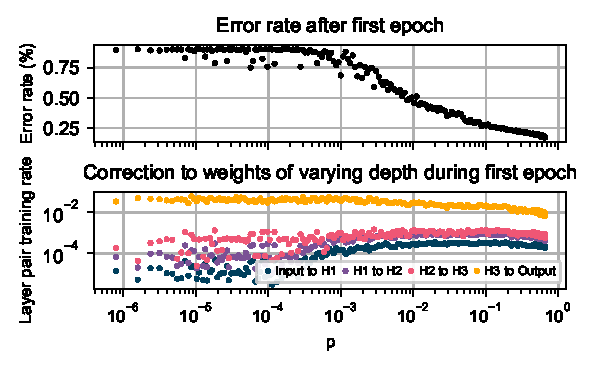
\includegraphics[width=\textwidth]{figures/MNIST_one_epoch_performance.pdf}
%\end{center}
%\caption{Behavior of our network (section \ref{sec:our_topology}) with varying $p$, during the first epoch of training. (top) The training error after one epoch. (bottom) Root-mean-square correction to weights in different layers during the first epoch. Observe that as $p$ is increased, the error rate decreases and the root-mean-square corrections to each layer become more-uniform.} \label{fig:mnist_1epoch}
%\end{figure}
%
%\begin{figure}[h!]
%\begin{center}
%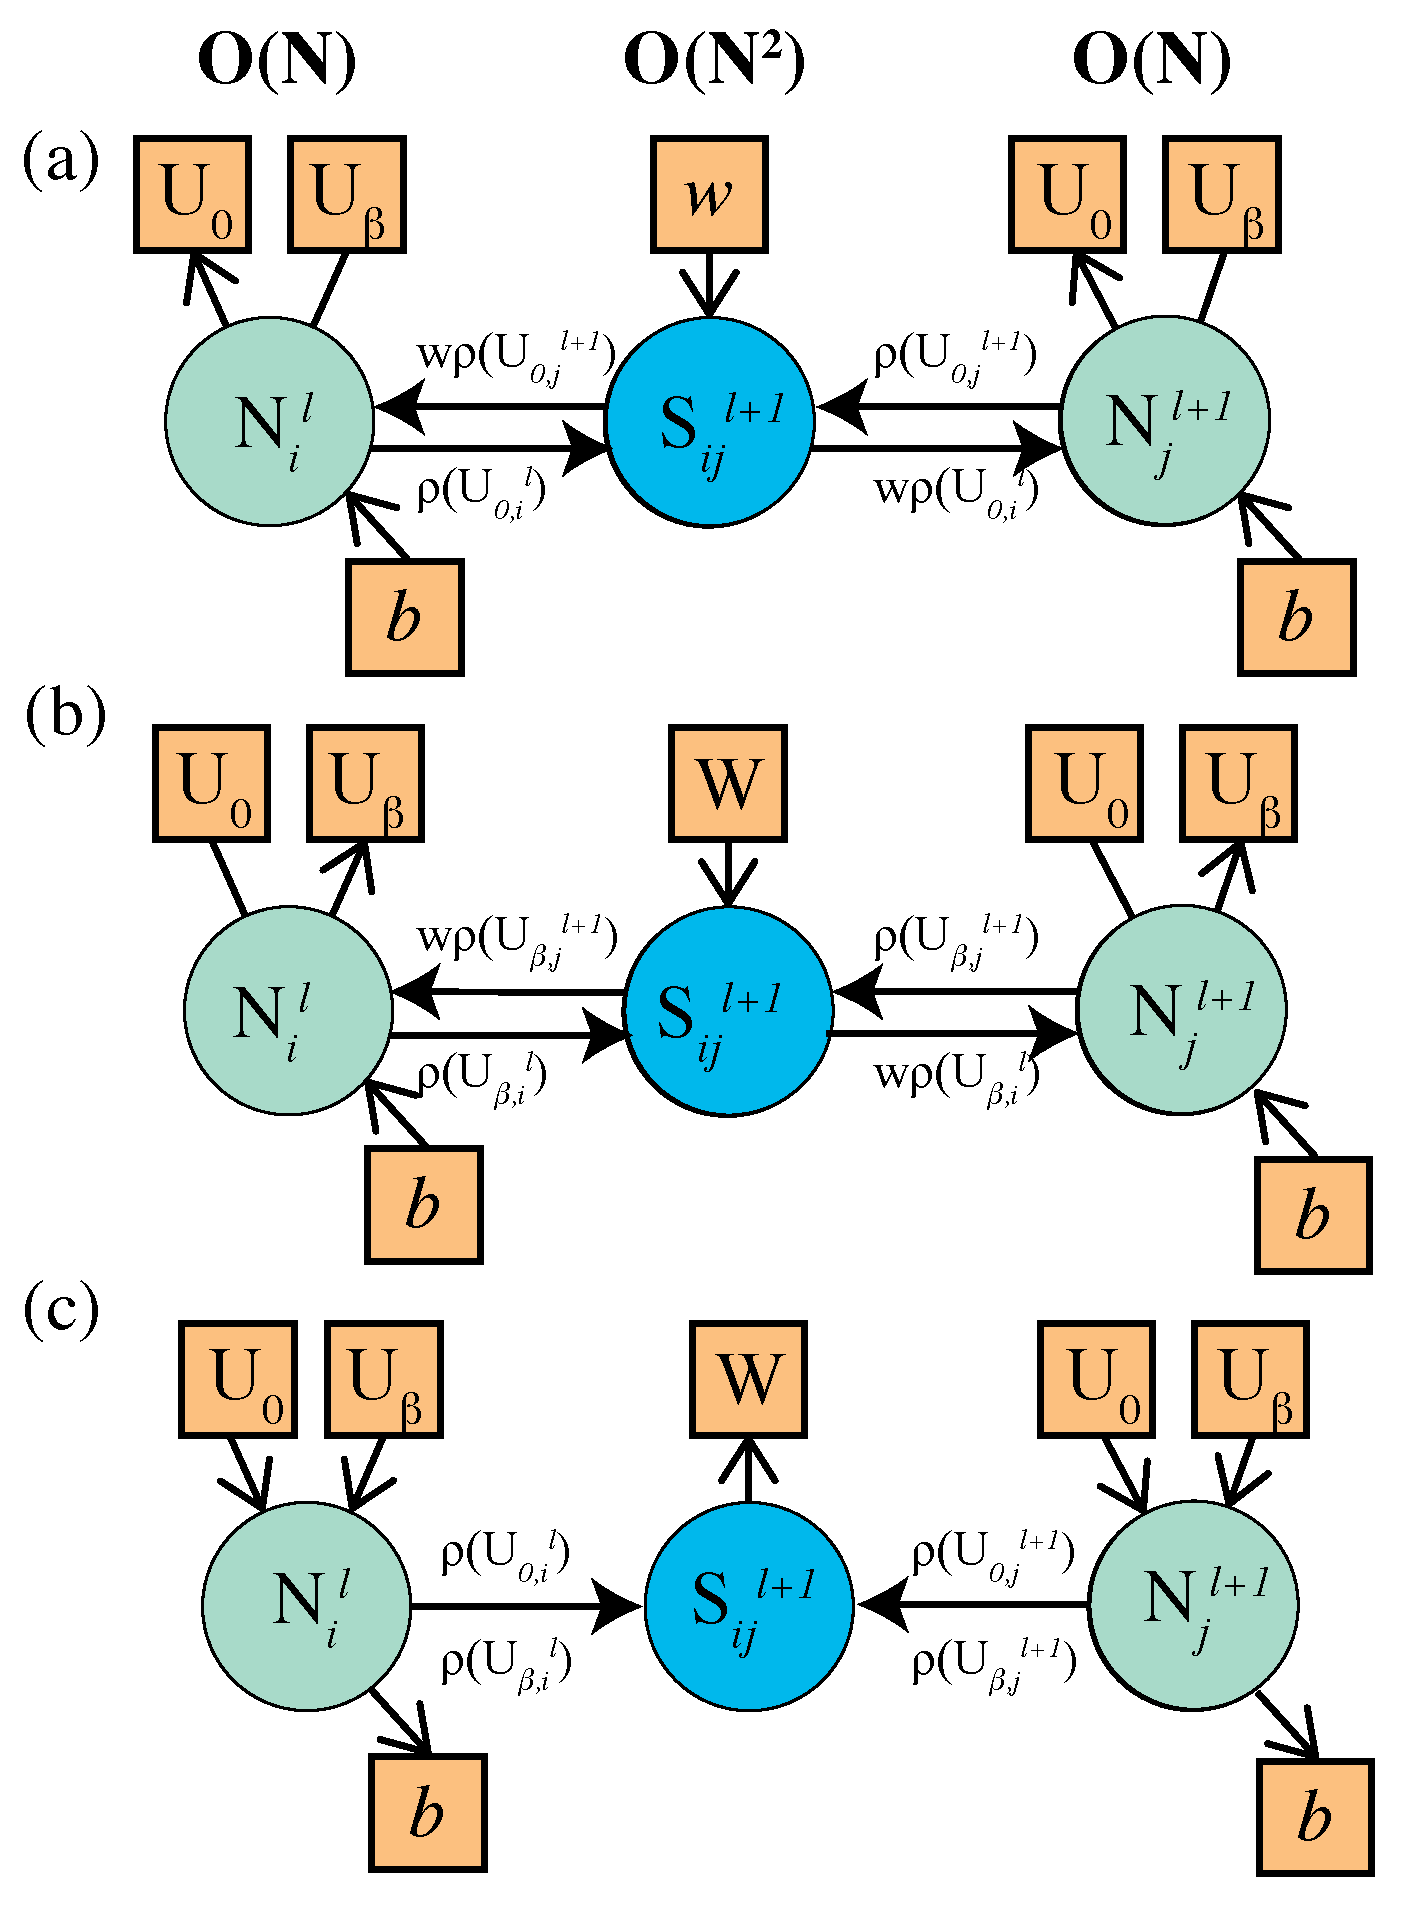
\includegraphics[width=10cm]{figures/eq_prop_sb.pdf}
%\end{center}
%\caption{Illustration of the functionality needed to implement equilibrium propagation in hardware. Yellow squares indicate a value that must be stored in memory for a subsequent phase. The circles indicate ($N$) neuron and ($S$) synapse devices with the associated functions described in the text. (a) The functionality required by the neurons and synapses in the free running phase. (b) The functionality of the neurons and synapses (except output neurons) in the weakly clamped phase. (c) The functionality of the neurons and synapses in the weight and bias update phase.} \label{fig:eq_prop}
%\end{figure}
%
%\begin{figure}[h!]
%\begin{center}
%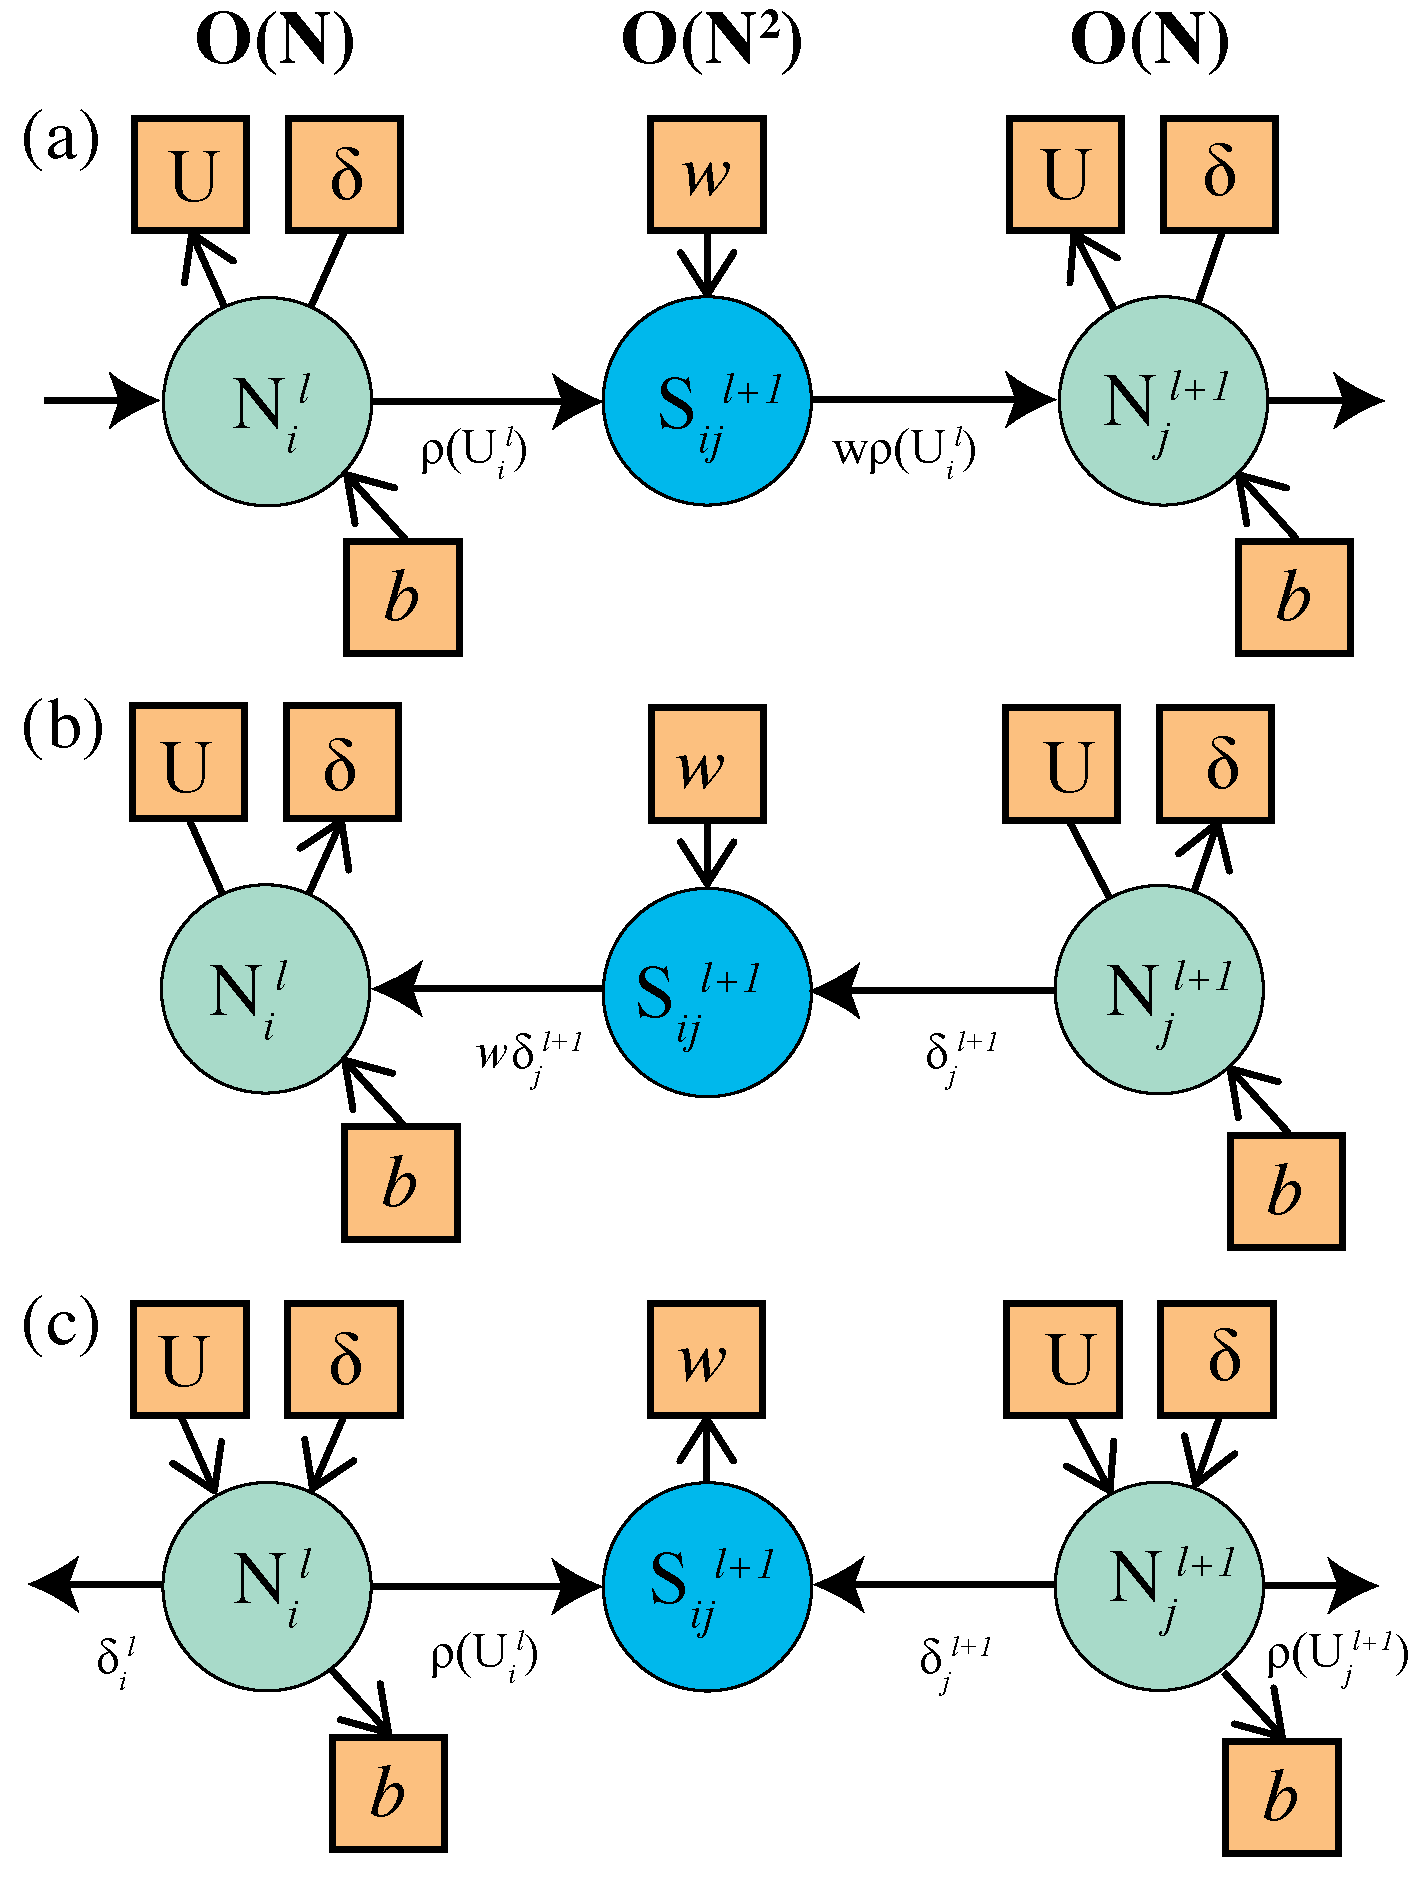
\includegraphics[width=10cm]{figures/back_prop_sb.pdf}
%\end{center}
%\caption{Illustration of the functionality needed to implement backpropagation in hardware. Yellow squares indicate a value that must be stored in memory for a subsequent phase. The circles indicate ($N$) neuron and ($S$) synapse devices with the associated functions described in the text. (a) The functionality required by the neurons and synapses in the forward pass phase. (b) The functionality of the neurons and synapses (except the last layer of neurons) in the backpropagation phase. (c) The functionality of the neurons and synapses in the weight and bias update phase.} \label{fig:back_prop}
%\end{figure}
%
%%\begin{figure}[h!]
%%\begin{center}
%%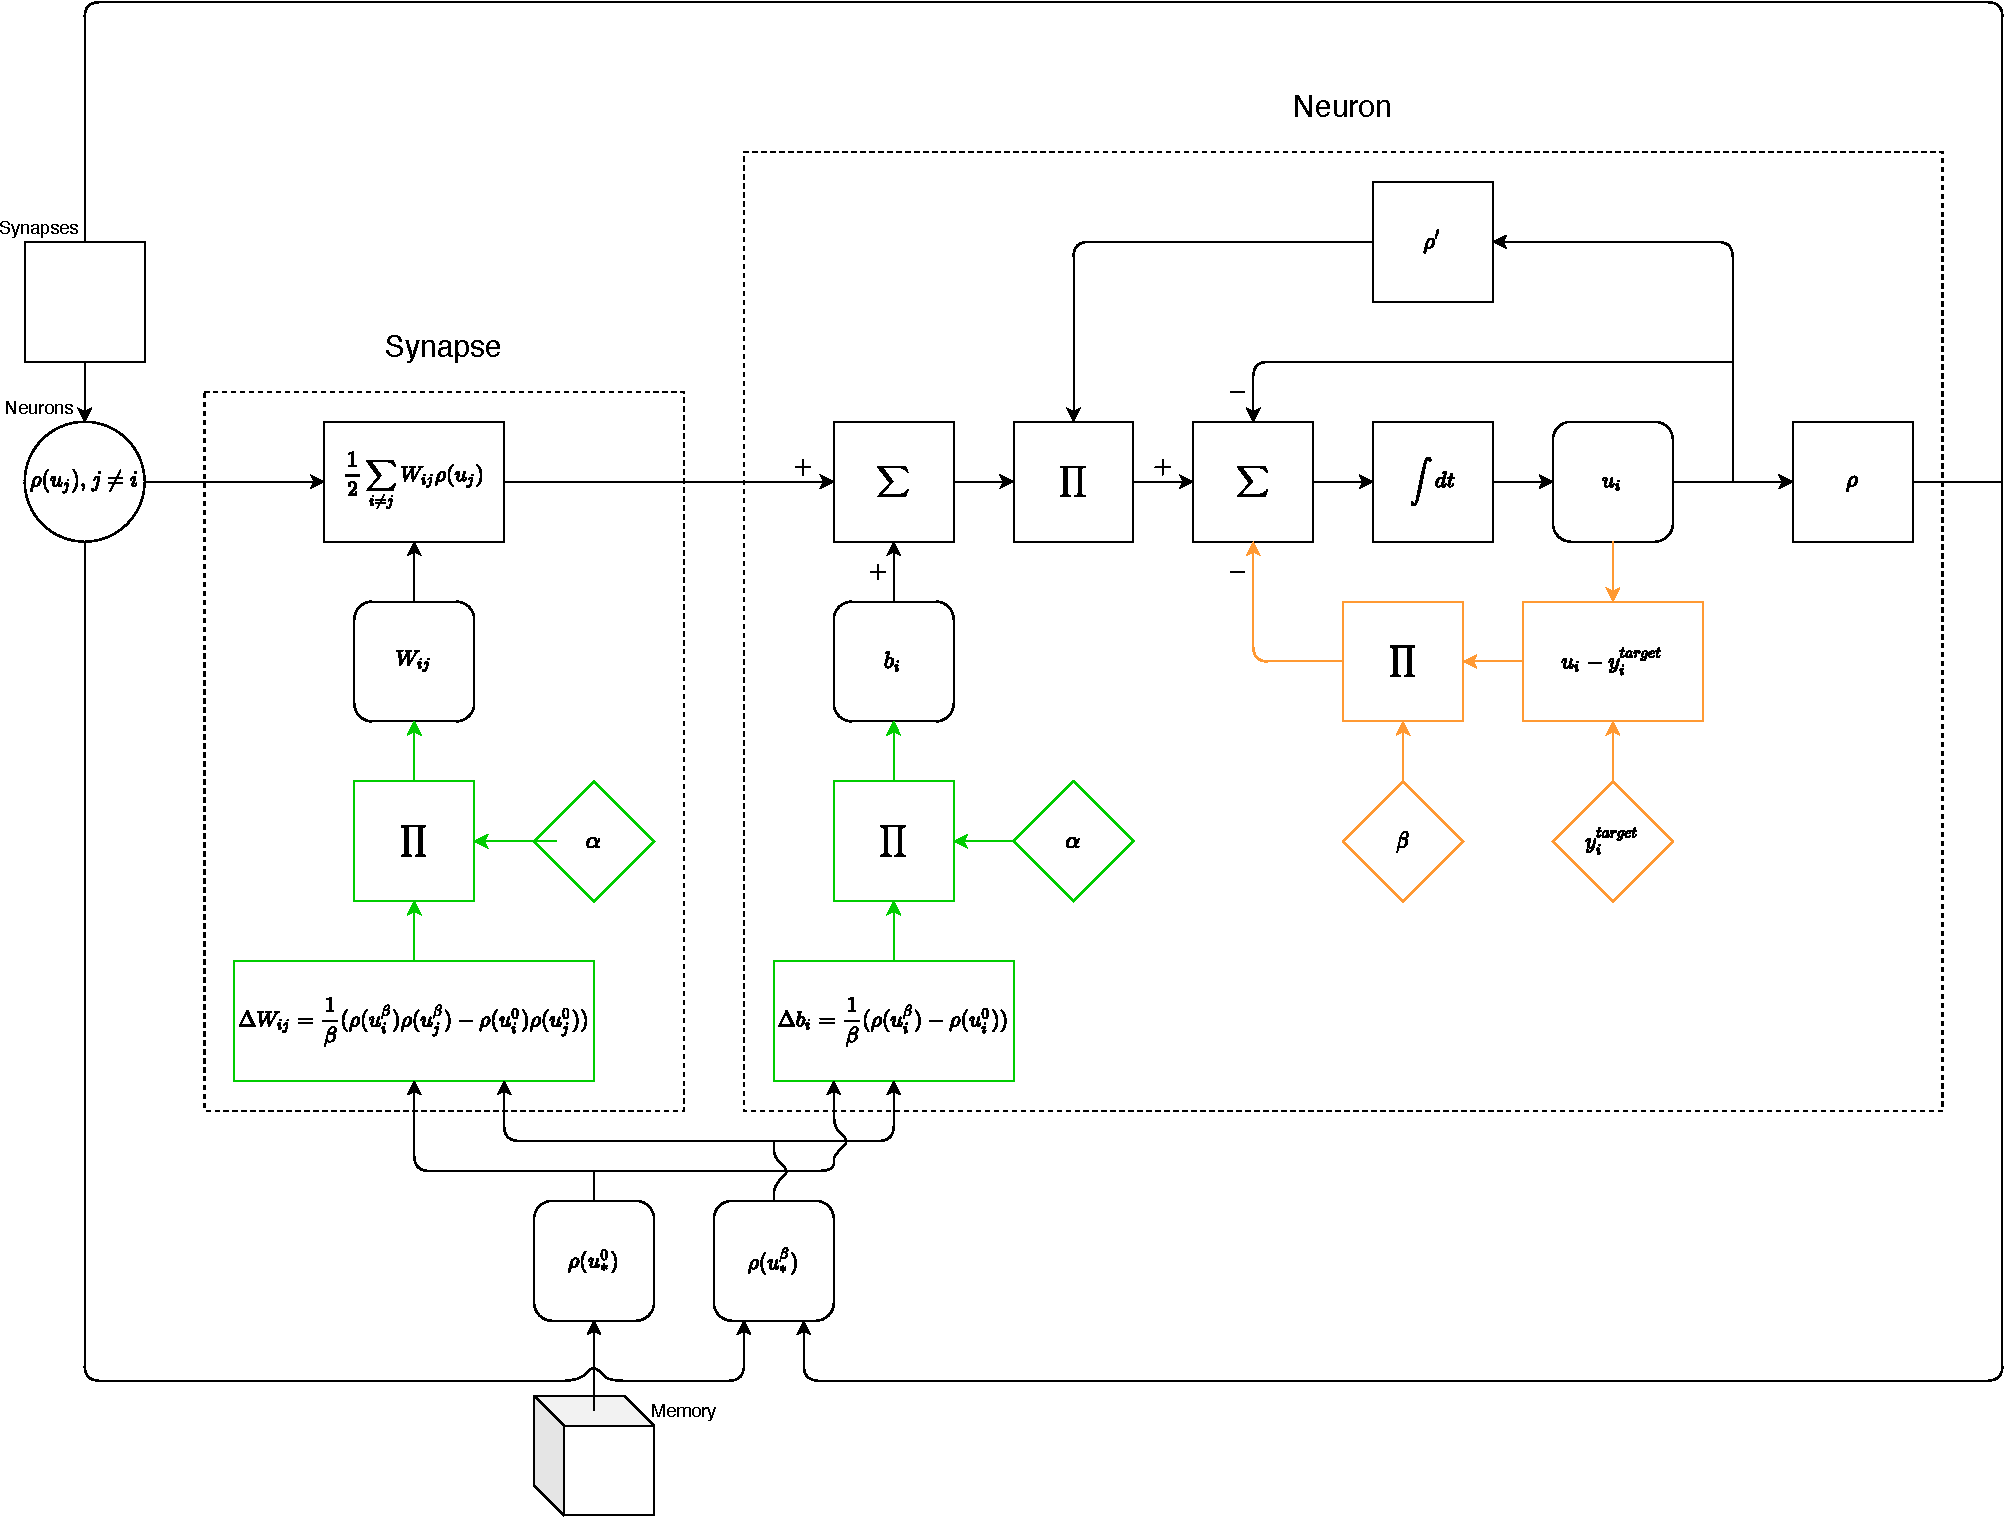
\includegraphics[width=\textwidth]{figures/eqp_bd.pdf}
%%\end{center}
%%\caption{Illustration of the functionality needed to implement equilibrium propagation in hardware. Black lines denote functionality needed in the free phase. Green lines denote functionality to correct parameters. Orange lines denote functionality needed only by output neurons, that is unique to the weakly-clamped phase. There is no functionality unique to the weakly-clamped phase that is needed by all neurons.} \label{fig:eqp_bd}
%%\end{figure}
%%\begin{figure}[h!]
%%\begin{center}
%%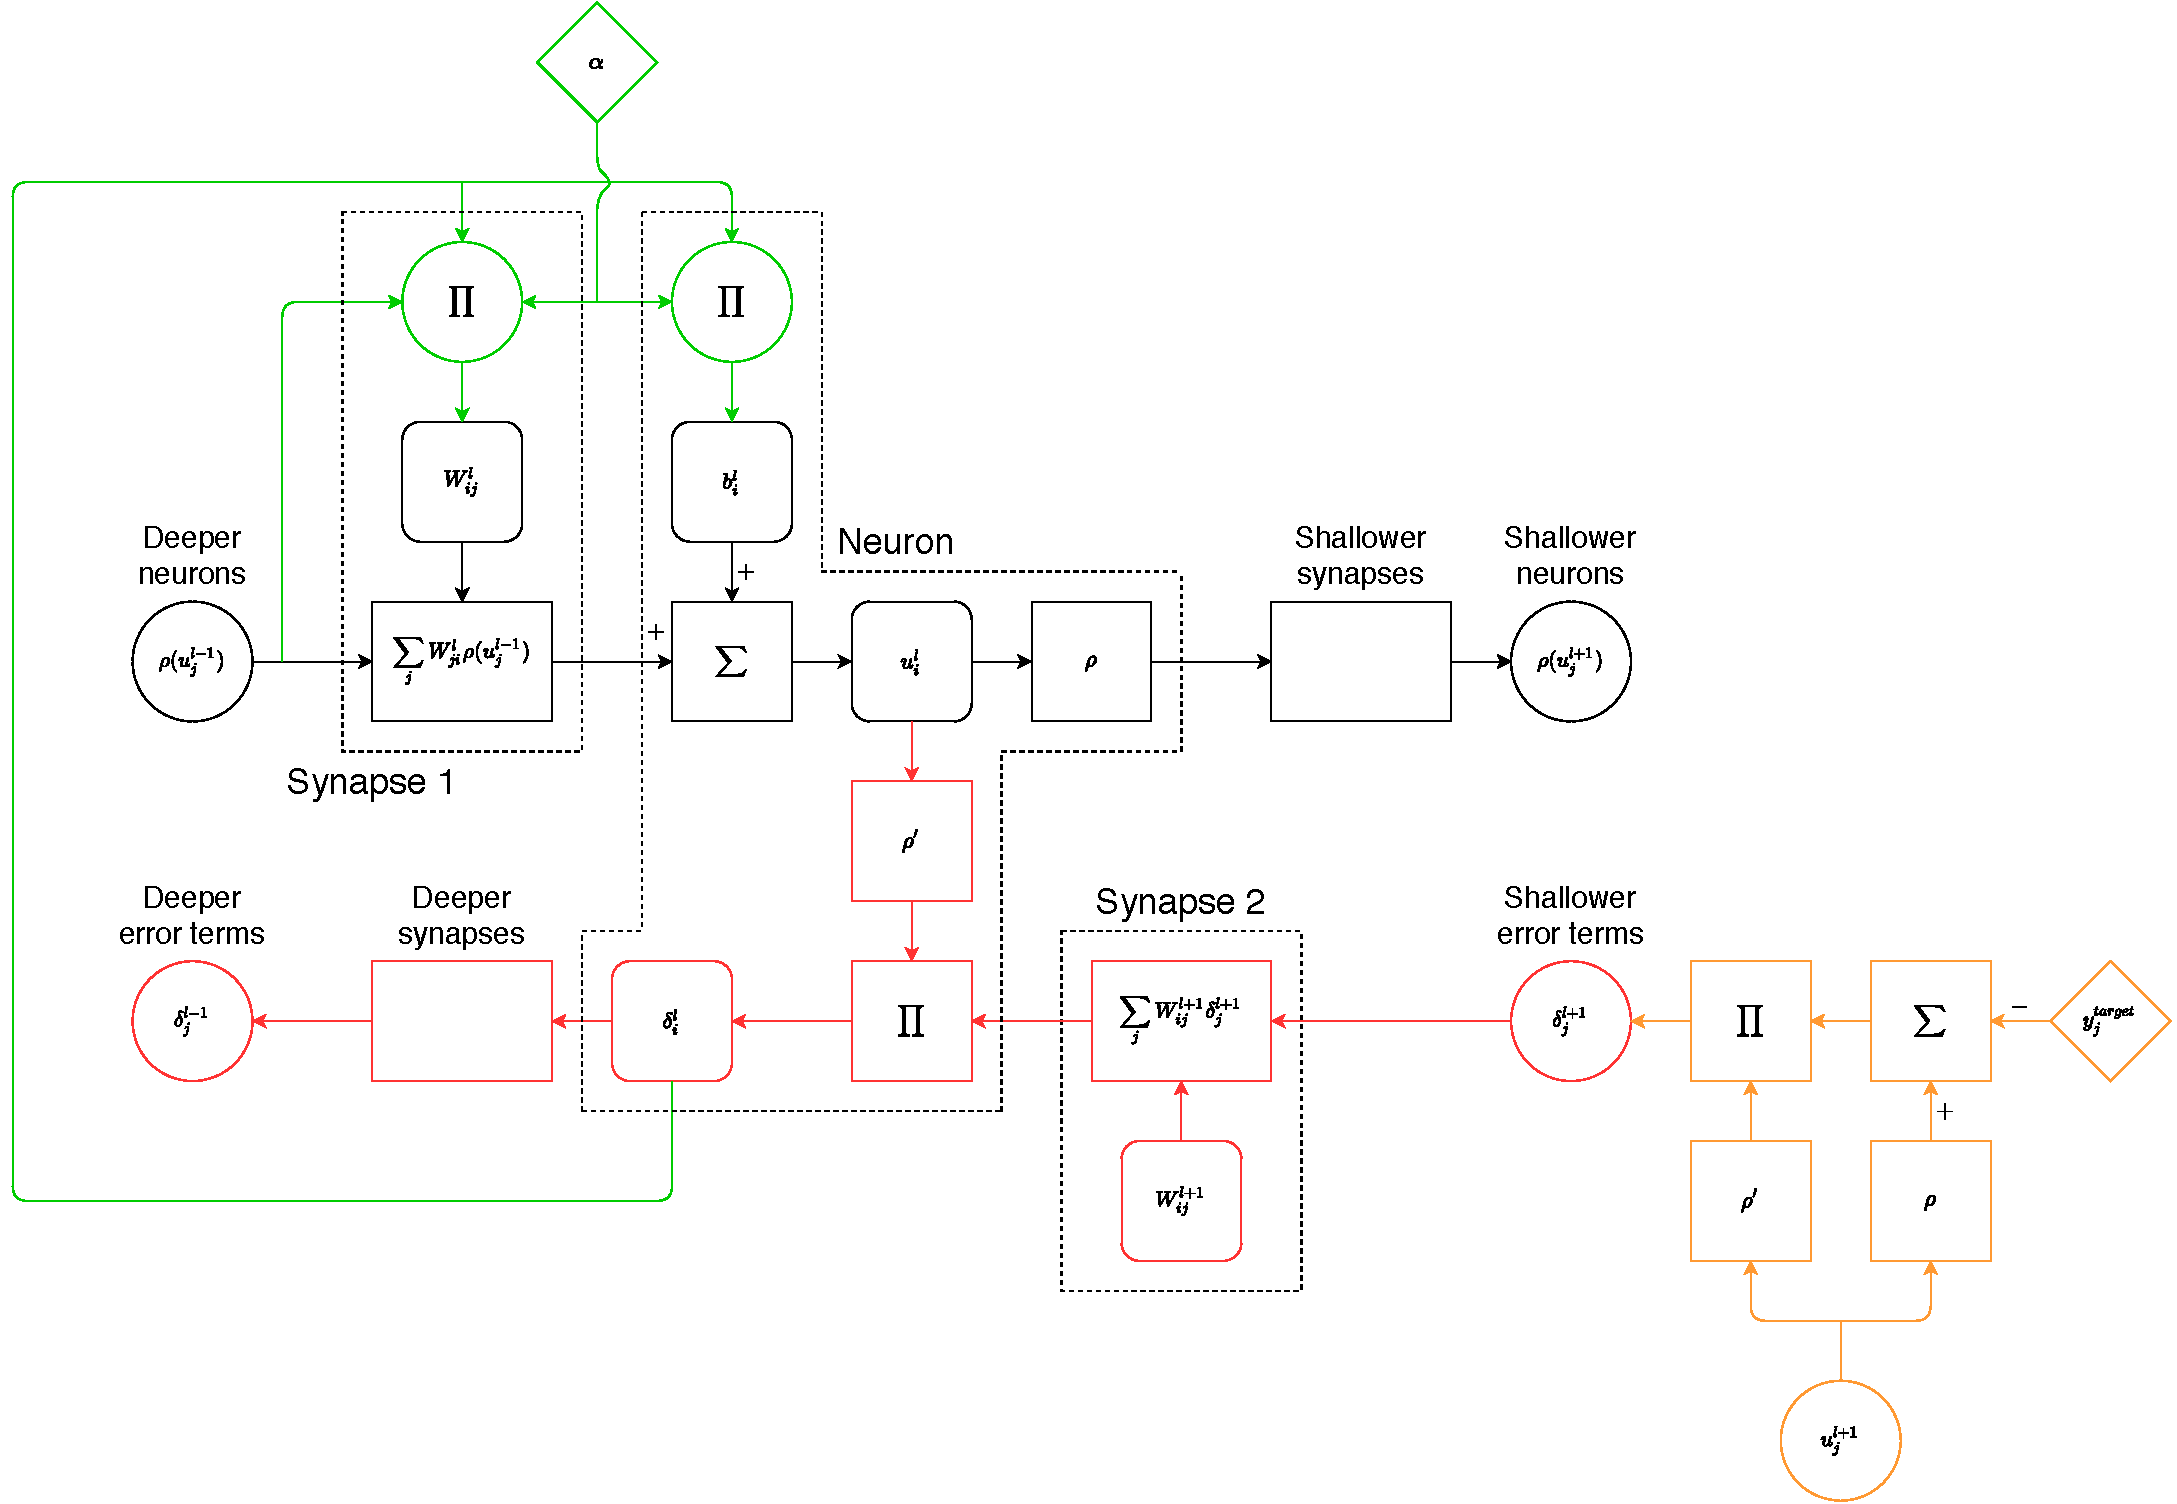
\includegraphics[width=\textwidth]{figures/backprop_bd.pdf}
%%\end{center}
%%\caption{Illustration of the functionality needed to implement backpropagation in hardware. Black lines denote functionality needed in the forwards phase. Green lines denote functionality to correct parameters. Red lines denote functionality unique to the backwards phase that is needed by all neurons. Orange lines denote functionality needed only by output neurons, that is unique to the backwards phase.} \label{fig:backprop_bd}
%%\end{figure}
%\clearpage
%\section*{Tables}
%\begin{table}[h!]
%\begin{center}
%\begin{tabular}{|L||L|L|}
%\hline
%&Backpropagation & Equilibrium Propagation \\ \hline\hline
%Number of distinct computations & 2 -- computations during forwards and backwards phases are distinct & $\approx 1$ -- hidden neurons perform same computation in both phases. Output neurons perform a similar but modified version of the same computation. \\ \hline
%Types of connections & Unidirectional to transmit activation to shallower neighbors and error to deeper neighbors & Bidirectional to each neighbor \\ \hline
%Memory & Space to store activation and error term for each neuron & Space to store free and weakly-clamped activations for each neuron \\ \hline
%Order of computations & Forwards propagation phase where layers are computed from deepest to shallowest; backwards propagation phase where layers are computed from shallowest to deepest; parameter update phase & Free phase where all neurons evolve simultaneously; weakly-clamped phase where all neurons evolve simultaneously; parameter update phase \\ \hline
%Nonlinear activation function & Yes & Yes \\ \hline
%Derivative of nonlinear activation function & Yes & Yes \\ \hline
%Correction computation & Corrections require dedicated circuitry unique from that implementing propagation & Corrections require dedicated circuitry unique from that implementing evolution \\ \hline
%\end{tabular}
%\end{center}
%\caption{Comparison of the capabilities a hardware neuron would need in order to implement backpropagation and equilibrium propagation.} \label{table:bp_eqp_contrast}
%\end{table}

\end{document}
